% !TEX encoding = UTF-8
% !TEX TS-program = pdflatex
% !TEX root = ../tesi.tex

\chapter{Il progetto: NFTLab}
\label{cap:nftlab}

%%%%%%%%%%%%%%%%%%%%%%%%%%%%%%%%%%%%%%%%%%%%%%%%%%%%%%%%%%%%%%%%%%%%%%%%%%%%%%%%%

% !TEX encoding = UTF-8
% !TEX TS-program = pdflatex
% !TEX root = ../../tesi.tex

\section{Analisi dei rischi}
Durante la fase di studio preliminare, ho proceduto all'identificazione dei rischi che potrebbero accadere durante la fase di sviluppo e, per ogni rischio identificato verrà fornita una descrizione, la probabilità che possa verificarsi e la sua Pericolosità. \\

\noindent La classificazione dei rischi ha seguito la seguente convenzione:
\begin{center}
  RI(S|R|T)[0-9]+
\end{center}
dove:
\begin{itemize}
  \item \textbf{S}: è la lettera con la quale si fa riferimento ad un rischio che si potrebbe incontrare durante il periodo di studio;
  \item \textbf{R}: è la lettera con la quale si fa riferimento ad un rischio che potrebbe essere causato dai requisiti;
  \item \textbf{T}: è la lettera con la quale si fa riferimento ad un rischio che potrebbe essere causato dalle tecnologie.
\end{itemize}

\noindent La pericolosità di ogni rischio è stata suddivisa in tre categorie:
\begin{itemize}
  \item \textbf{Impatto alto}: provoca uno sforamento significativo sulle ore previste ed è difficilmente risolvibile nel tempo di progetto;
  \item \textbf{Impatto medio}: provoca uno sforamento di qualche ora ed è risolvibile;
  \item \textbf{Impatto basso}: provoca uno sforamento trascurabile delle ore pianificate ed è facilmente risolvibile.
\end{itemize}

\begin{longtabu}{|X[1,c]|X[2,c]|X[0.8,c,m]|X[0.8,c,m]|}

  \hline

  \textbf{Codice identificativo} & \textbf{Descrizione} & \textbf{Probabilità} & \textbf{Pericolosità} \\

  \hline

  \risk{S} & Non comprensione di un argomento presentato durante il periodo di studio & Media & Media \\

  \hline

  \risk{R} & & &  \\

  \hline

  \risk{T} & Difficoltà nell'imparare il linguaggio Solidity & Media & Alta \\
  % \risk{T} & Difficoltà nell'imparare il linguaggio Solidity & &  \\

  \hline

  \caption{Analisi dei rischi}
\end{longtabu}


%%%%%%%%%%%%%%%%%%%%%%%%%%%%%%%%%%%%%%%%%%%%%%%%%%%%%%%%%%%%%%%%%%%%%%%%%%%%%%%%%

% !TEX encoding = UTF-8
% !TEX TS-program = pdflatex
% !TEX root = ../../tesi.tex

\section{Studio preliminare}
Durante la fase di studio preliminare ho dovuto apprendere tutte le nozioni teoriche che stanno alla base del funzionamento della \textbf{tecnologia \textit{blockchain}} e, in seguito, alla base delle \textit{blockchain} \textbf{Ethereum} e \textbf{Hotmoka}, con i relativi linguaggi per la scrittura di \textit{smart contract}.

\subsection{Cos'è la blockchain}
La \textit{blockchain} è una nuova tipologia di registro distribuito strutturato come una catena di blocchi contenenti le transazioni. Fa parte, perciò, della più ampia famiglia delle tecnologie di \textbf{\textit{Distributed Ledger}}, ossia sistemi che si basano su un registro distribuito che può essere letto e modificato da più nodi di una rete.

In più, un'altra caratteristica molto importante della \textit{blockchain} è il fatto di essere \textit{permissionless}, ovvero chiunque può connettersi alla rete e far parte del complesso sistema che la regola. Questo rende tutto molto più complesso dato che, reti come questa, hanno bisogno di un sistema di consenso molto più forte, rispetto a reti \textit{permissioned}, per assicurare la validità e il funzionamento corretto del sistema. \\

\noindent Le caratteristiche della tecnologia \textit{blockchain}, riassumendo, sono le seguenti:
\begin{itemize}
  \item \textbf{Decentralizzazione}: le informazioni vengono registrate distribuendole tra più nodi per garantire sicurezza informatica e resilienza dei sistemi;
  \item \textbf{Tracciabilità dei trasferimenti}: ciascun elemento sul registro è tracciabile in ogni sua parte e se ne può risalire all’esatta provenienza;
  \item \textbf{Disintermediazione}: le piattaforme consentono di gestire le transazioni senza intermediari, ossia senza la presenza di enti centrali fidati;
  \item \textbf{Trasparenza e verificabilità}: il contenuto del registro è trasparente e visibile a tutti ed è facilmente consultabile e verificabile;
  \item \textbf{Immutabilità del registro}: una volta scritti sul registro, i dati non possono essere modificati senza il consenso della rete;
  \item \textbf{Programmabilità dei trasferimenti}: possibilità di programmare determinate azioni che vengono effettuate al verificarsi di certe condizioni. Questa caratteristica non è presente nella \textit{blockchain} BitCoin.
\end{itemize}

Per comprendere al meglio come funzionano tutti questi meccanismi, introduciamo ed approfondiamo la prima \textit{blockchain} che sia mai stata creata, ovvero BitCoin. \\

\textbf{BitCoin} è nata alla fine del 2009 quando Satoshi Nakamoto, una persona o un gruppo di persone la cui identità è tutt'ora ignota, pubblica un \textit{white paper} spiegando la sua idea di moneta virtuale crittografica \textit{peer-to-peer} senza intermediari. Di seguito verranno approfonditi i concetti principali di questa tecnologia.

% \begin{figure}[h!]
%   \centering
%   
\includegraphics[width=0.2\textwidth]{capitolo3/bitcoin-logo.png}
%   \caption{Logo di BitCoin}
%   \textbf{Fonte}: \href{https://bitcoin.org/it/}{https://bitcoin.org}
% \end{figure}

\paragraph{Il wallet}
Il concetto di \textit{wallet}, o portafoglio in italiano, è importantissimo e permette a chiunque di interagire con la \textit{blockchain}. Consiste in un applicativo \textit{software} che consente la compravendita della criptovaluta BitCoin.

% Il \textit{wallet} ha lo stesso compito del codice IBAN di un conto corrente.

Ogni \textit{wallet} ha un indirizzo, il quale viene creato attraverso un processo di manipolazione di una chiava privata che si ottiene producendo un numero casuale tra \( 0 \) e \( 2^{256}-1 \), sfruttando un generatore di numeri casuali uniformemente distribuito, dove vengono utilizzati algoritmi che generano numeri con la stessa probabilità. Questa chiave privata viene creata localmente ed è importantissima in quanto tutte le transazioni vengono firmate digitalmente con essa e permette l'accesso al proprio \textit{wallet}. Se viene rubata non si può fare altro, se non rassegnarsi d'aver perso tutti i propri BitCoin.

Dalla chiave privata attraverso l'applicazione della funzione di ECDSA-512, viene ottenuta la chiave pubblica e, in seguito, dalla chiave pubblica si ottiene l'indirizzo del \textit{wallet} applicando la funziona di hash RipeMD160 e convertendo il risultato in \textit{base58} per una migliore comprensione di quest'ultimo. Inoltre dall'indirizzo del \textit{wallet} sono state rimosse tutte le lettere o numeri ambigui come lo sono lo zero e la lettera O.

\begin{figure}[tbh!]
  \centering
  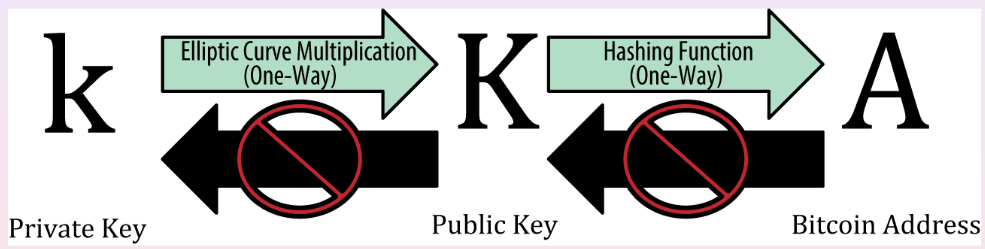
\includegraphics[width=\textwidth]{capitolo3/studio-preliminare/bitcoin-keys.png}
  \caption{Flusso di generazione del \textit{wallet} in BitCoin}
  \textbf{Fonte}: \href{https://github.com/spoto/blockchain-course/blob/master/Bitcoin}{https://github.com/spoto/blockchain-course/blob/master/Bitcoin}
\end{figure}

Data l'attenzione che bisogna dedicare alla sicurezza della chiave privata sono nate molte tecniche per facilitarne la memorizzazione. Una di queste tecnologie così importanti sono i \textbf{Deterministic Wallet}, grazie ai quali non bisognerà ricordarsi la chiave privata associata ad ogni \textit{wallet} che una persona ha, ma ci sarà una \textit{Master Private Key} da cui si potranno derivare in maniera deterministica tutte le altre chiavi private, dalle quale si otterranno gli indirizzi dei \textit{wallet}. 

Un'altra soluzione che sta sempre più prendendo piede è l'utilizzo delle \textit{12 words}, dove la chiave privata viene associata a 12 parole che vengono pescate da un vocabolario di circa 2048 parole. In seguito verrà anche associata ad una password personale e, la combinazione di quest'ultima con le dodici parole permette di ricondursi alla chiave privata originale. 

\paragraph{Come si svolge una transazione}
Per comprendere al meglio come si svolge una transazione in BitCoin dobbiamo prima apprendere come vengono gestiti i bilanci dei vari \textit{wallet}. BitCoin stravolge il paradigma applicato ai sistemi bancari attuali dove si ha una determinata somma di denaro e a questa viene sottratto o aggiunto un valore in base alla situazione. Il modello utilizzato da BitCoin, invece, si chiama \textbf{UTXO (\textit{Unspent Transaction Output})} e non si possederà più una certa quantità di denaro, ma bensì le transazioni non ancora spese che hanno un mio \textit{wallet} come destinatario. Un \textit{wallet}, perciò, ha il compito di registrare e tenere conto di tutte le transazioni assegnate a lui. Per comprare qualsiasi bene attraverso la moneta BitCoin bisognerà utilizzare le transazioni possedute, le quali non possono essere frazionate. Il denaro di resto, ovviamente, ritornerà sotto forma di un'altra transazione.

\begin{figure}[h!]
  \centering
  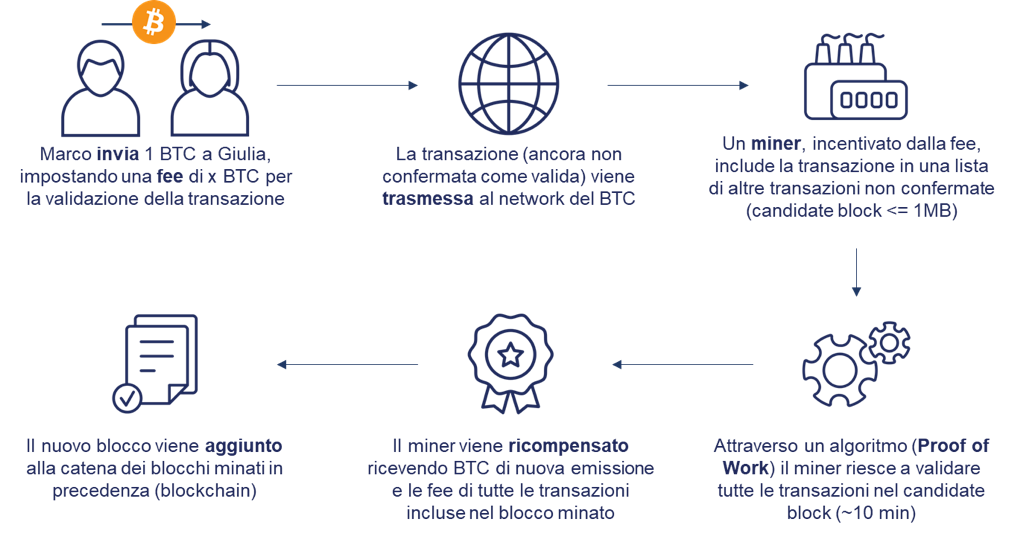
\includegraphics[width=\textwidth]{capitolo3/studio-preliminare/bitcoin-transaction.png}
  \caption{Esecuzione di una transazione in BitCoin}
  \textbf{Fonte}: \href{https://www.focusmgmt.it/knowledge/innovazione-nella-blockchain-il-lightning-network/}{https://www.focusmgmt.it/knowledge/innovazione-nella-blockchain-il-lightning-network}
\end{figure}

Quando si verifica una transazione questa viene diffusa a tutti i \textit{peer} della rete per essere elaborata. A questo punto entrano in gioco i \textit{\textbf{miner}}, ovvero \textit{peer} che hanno il compito di validare le transazioni ed inserirle nella \textit{blockchain} all'interno di nuovi blocchi. Ogni \textit{miner} fa questo per ottenere la commissione, che viene inserita dal mittente del pagamento, e una certa quantità di BitCoin che vengono generati direttamente dalla \textit{blockchain}.

Appena un \textit{miner} riceve una transazione la colloca dentro la \textit{mining pool}, ovvero un grande contenitore dove vengono posizionate tutte le transazioni che ha ricevuto e che deve elaborare. Di solito, per la complessità di questo processo, il \textit{miner} seleziona solo quelle con la commissione più alta in modo da massimizzare il ricavo.

In seguito avviene la creazione del blocco con le transazioni scelte e, cosa più importante, inizia  il processo di \textit{proof of work}. Il \textbf{\textit{proof of work}} consiste in un processo che obbliga il minatore ad allegare al blocco la prova di aver compiuto un lavoro. Questo lavoro consiste nel trovare un numero, chiamato \textit{\textbf{nonce}}, che inserito dentro il \textit{header} del blocco faccia si che il suo hash sia minore di un valore intrinseco della rete, variabile in un determinato intervallo, chiamato \textit{difficulty}. È un lavoro molto pesante e serve a non incoraggiare la creazione di blocchi falsi e malevoli. Attualmente, per come è stata impostata la \textit{difficulty} della rete, un minatore ci mette circa 10 minuti a produrre un blocco valido.

\begin{figure}[h!]
  \centering
  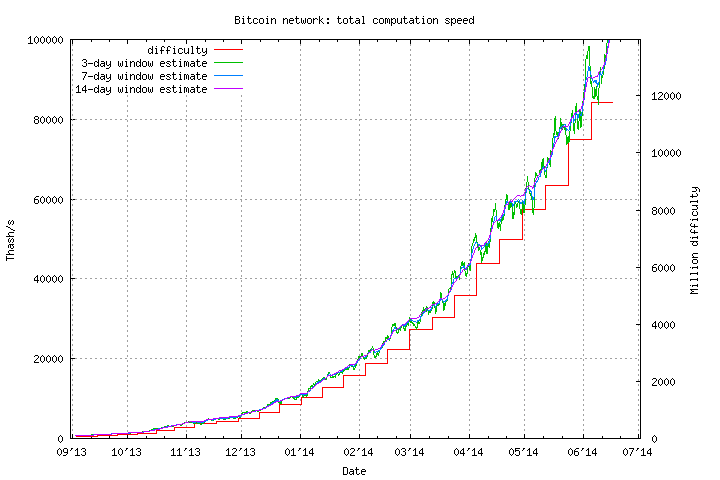
\includegraphics[width=0.9\textwidth]{capitolo3/studio-preliminare/bitcoin-difficuly.png}
  \caption{La crescente difficoltà del minare BitCoin causata dalla scoperta di tecnologie sempre più veloci}
  \textbf{Fonte}: \href{https://blog.ethereum.org/2014/06/19/mining/}{https://blog.ethereum.org/2014/06/19/mining/}
\end{figure}

Quando avrà ottenuto il blocco valido, lo condividerà nella rete per informare tutti su quali transazioni ha validato e condividere lo stato della sua \textit{blockchain} interna. Gli altri \textit{peer} valideranno il blocco controllando che tutti i campi siano corretti e lo accetteranno in tal caso. A questo punto il \textit{miner} potrà prendere la sua ricompensa composta dalle commissioni delle transazioni che ha validato e la moneta emessa dalla \textit{blockchain}. Dato che la validazione delle transazioni è un processo mutualmente esclusivo, ma tutti possono concorrere per la loro validazione, quando viene informata la rete della creazione di un nuovo blocco valido tutti gli altri \textit{peer} controllano le transazioni che sono al suo interno e, nel caso in cui ne sia presente una su cui stanno lavorando, dovranno scartare il blocco che stanno creando e ricominciarlo da capo non percependo alcuna ricompensa.

\paragraph{Composizione di un blocco in BitCoin}

Un blocco della \textit{blockchain} BitCoin è molto semplice ma complesso allo stesso tempo. Le parti principali che lo compongono sono:

\begin{itemize}
  \item \textbf{\textit{Header} del blocco}:
  \begin{itemize}
    \item \textbf{Hash del blocco precedente};
    \item \textbf{\textit{Timestamp}}: data di creazione del blocco;
    \item \textbf{\textit{Difficulty}}: difficoltà che è stata assegnata al blocco. Serve al processo di \textit{proof of work};
    \item \textbf{\textit{Nonce}}: prova di aver compiuto un lavoro che si porta dietro il blocco;
    \item \textbf{\textit{Merkle root}}: hash della radice del \textit{Merkle Tree} delle transazioni.
  \end{itemize}
  
  \item \textbf{Transazioni}: dove sono presenti tutte le transazioni validate nel blocco.
\end{itemize}

\begin{figure}[h!]
  \centering
  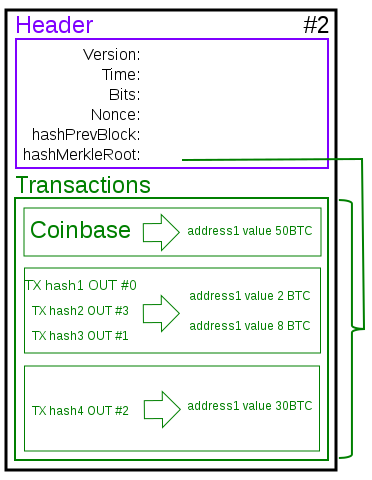
\includegraphics[width=0.4\textwidth]{capitolo3/studio-preliminare/bitcoin-block-structure.png}
  \caption{Composizione di un blocco in BitCoin}
  \textbf{Fonte}: \href{https://github.com/spoto/blockchain-course/blob/master/Bitcoin}{https://github.com/spoto/blockchain-course/blob/master/Bitcoin}
\end{figure}

Un \textbf{\textit{Merkle Tree}} è una struttura dati che la tecnologia \textit{blockchain} utilizza per la verifica della validità di una transazione con modalità \textit{Zero knowledge proof}.

% \clearpage
\begin{figure}[h!]
  \centering
  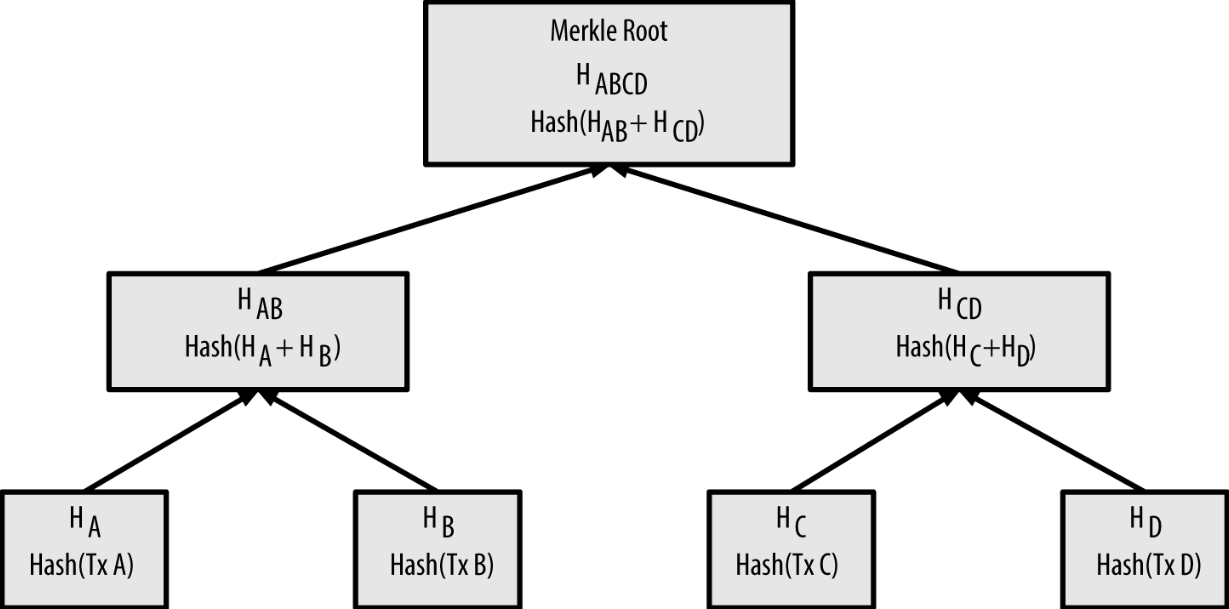
\includegraphics[width=0.9\textwidth]{capitolo3/studio-preliminare/bitcoin-merkle-tree.png}
  \caption{Esempio di Merkle Tree}
  \textbf{Fonte}: \href{https://github.com/spoto/blockchain-course/blob/master/Bitcoin}{https://github.com/spoto/blockchain-course/blob/master/Bitcoin}
\end{figure}

Consiste in un albero binario sempre bilanciato nel quale alle foglie sono presenti tutte le transazioni interne al blocco. Ogni nodo non foglia avrà come valore il hash del hash dei suoi figli. In questo modo un qualsiasi \textit{peer} può verificare che una transazione sia valida e presente all'interno di un determinato blocco chiedendo semplicemente ad un \textit{full node} (nodo con tutta la \textit{blockchain} memorizzata) di verificarla. Il \textit{full node} gli invierà le transazioni che permetteranno di risalire al \textit{Merkle root} dell'albero a partire dalla transazione che vuole verificare, semplicemente eseguendo l'operazione di hash tra i blocchi ricevuti. Come funzione di \textit{hashing} viene utilizzata SHA256 anche nelle \textit{blockchain} che tratterremo di seguito.

% \clearpage
\begin{figure}[h!]
  \centering
  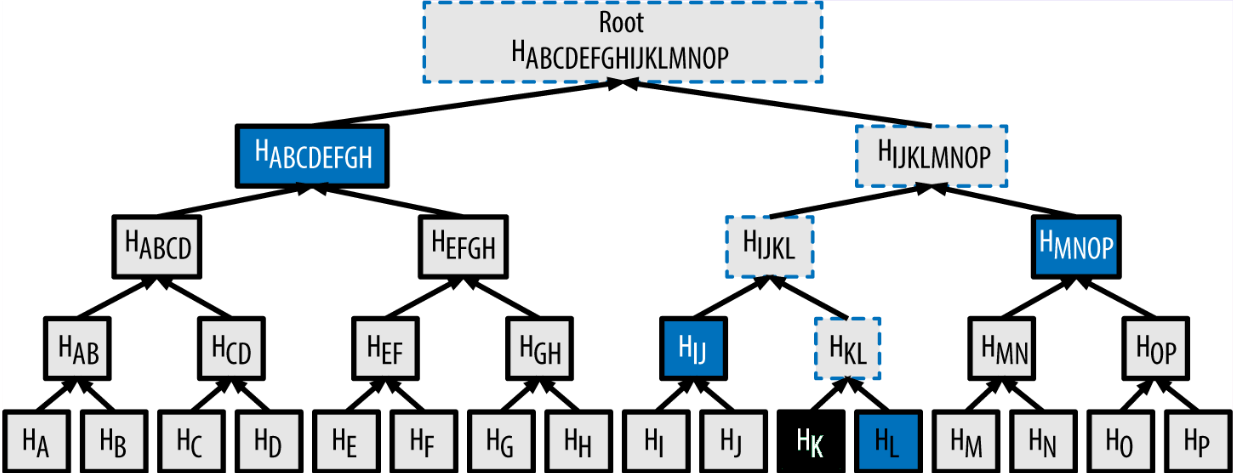
\includegraphics[width=0.9\textwidth]{capitolo3/studio-preliminare/bitcoin-merkle-tree-verify.png}
  \caption{Esempio di verifica di una transazione in un Merkle Tree}
  \textbf{Fonte}: \href{https://github.com/spoto/blockchain-course/blob/master/Bitcoin}{https://github.com/spoto/blockchain-course/blob/master/Bitcoin}
  \label{fig:merkle-tree-verify}
\end{figure}

Ad esempio, come si può vedere in figura \ref{fig:merkle-tree-verify}, per verificare che la transazione H\textsubscript{k} sia effettivamente in un blocco, il \textit{peer} chiederà ad un \textit{full node} di mandargli tutte le transazioni colorate in blu. A questo punto il \textit{peer} richiedente potrà ottenere tutti i nodi tratteggiati di blu fino ad arrivare alla radice, per poi confrontarla con il hash del \textit{Merkle root} presente nel blocco. Se corrispondono significa che la transazione H\textsubscript{k} è presente in quel blocco. 

\paragraph{Le diramazioni in BitCoin}
Essendo la \textit{blockchain} un sistema distribuito, deve tenere in considerazione il problema dell'inconsistenza dei dati e delle possibili diramazioni della storia delle transazioni che si creano ogni secondo.

Non è rara la situazione in cui un blocco sia il precedente di due blocchi. BitCoin risolve questo problema mantenendo come storia principale quella con più blocchi e non accettando più aggiunte di nuovi blocchi che hanno come blocco precedente un blocco di una diramazione non più valida.

% \paragraph{Sicurezza nella Blockchain}
% L'attacco più famoso e pericoloso che si possa attuare in BitCoin, o nelle \textit{blockchain} che utilizzano \textit{proof-of-work} come algoritmo per il consenso, consiste nell'\textbf{attacco del 51\%}. Questo attacco avviene quando una persona, o un gruppo di persone, detiene il potere computazionale del 51\%. Salta così il concetto di rete decentralizzata, infatti avendo il controllo della maggioranza della potenza di calcolo si potrà decidere aggiungere nuovi blocchi, manipolare le operazioni bidirezionali e rifiutarsi di confermare le nuove transazioni. 

% Attraverso questo attacco è possibile eseguire anche il \textbf{\textit{double spending}}, ovvero illudere il sistema di non aver speso una transazione e riutilizzarla effettuare un altro acquisto.

% C'è da dire che non si è mai verificato un caso di questo attacco in un \textit{blockchain} grande come lo è BitCoin o lo può essere Ethereum, visto che sono troppo distribuite nel mondo e risulta quasi impossibile riuscire ad avere il 51\% della potenza di calcolo totale.  

%%%%%%%%%%%%%%%%%%%%%%%%%%%%%%%%%%%%%%%%%%%%%%%%%%%%%%%%%%%%%%%%%%%%%%%%%%%%%%%%%%% 

\subsection{La blockchain Ethereum}
La \textit{blockchain} Ethereum è nata nel 2014 da un'idea di Vitalik Buterin e Gavin Wood. Quello che volevano e hanno creato è una \textit{blockchain} programmabile attraverso programmi chiamati \textit{smart contract} che possono essere installati all'interno di blocchi della \textit{blockchain}. \\

Sotto tanti aspetti non si differenzia di molto da BitCoin per quanto riguarda il funzionamento del consenso, la composizione dei blocchi e la creazione del \textit{wallet}, tranne per qualche funzione crittografica utilizzata. La grande differenza rispetto a BitCoin è che viene introdotto il concetto di stato di un blocco. Infatti se prima ogni transazione in BitCoin corrispondeva alla generazione di una \textit{UTX}, ora viene generalizzato questo concetto corrispondendo ad un cambiamento dello stato di un blocco.

% \begin{figure}[h!]
%   \centering
%   
\includegraphics[width=0.1\textwidth]{capitolo3/ethereum-logo.png}
%   \caption{Logo di Ethereum}
%   \textbf{Fonte}: \href{https://ethereum.org/it}{https://ethereum.org}
% \end{figure}

\paragraph{Il concetto di smart contract} \label{par:ethereum.smart-contract}
Uno \textit{smart contract} è un programma installabile all'interno di un blocco di una \textit{blockchain} con il quale è permesso scambiare valuta o modificare lo stato di entità presenti, in modo trasparente senza conflitti evitando servizi di terze parti. \\

\noindent Le caratteristiche di uno \textit{smart contract} sono:
\begin{itemize}
  \item \textbf{Immutabilità}: il codice di uno \textit{smart contract} caricato in \textit{blockchain} non può essere modificato;
  \item \textbf{Irrevocabilità}: non può essere cancellato;
  \item \textbf{Deterministico}: non possono essere utilizzati metodi non deterministici, come la generazione di numeri casuali, perché ogni operazione deve essere ripetibile in caso di riallineamento della stato;
  \item \textbf{Terminabile}: anche se i linguaggi di programmazione con cui si possono scrivere \textit{smart contract} sono \gls{turing completi}, sono stati applicati dei sistemi per far si che termini sempre. Questo perché non si possono fermare dei \textit{peer} della rete per l'esecuzione di uno \textit{smart contract} che non termina;
  \item \textbf{Isolato}: tutti i cambiamenti di stato devono essere eseguiti in un ambiente indipendente dal \textit{peer} della rete. Per questo esiste la \textit{EVM} (\textit{Ethereum Virtual Machine}).
\end{itemize}

\noindent Con uno \textit{smart contract} si può:
\begin{itemize}
  \item far eseguire computazioni ai \textit{peer} della rete distribuita della \textit{blockchain};
  \item mantenere la persistenza di dati;
  \item trasferire soldi (Ether) da un EOA a un qualsiasi altro EOA.
\end{itemize}

Per rendere sempre terminabile uno \textit{smart contract}, Ethereum ha introdotto il concetto di \textit{Gas limit} e \textit{Gas price}.
Il \textbf{\textit{Gas limit}} è la massima quantità di \textit{Gas} che si è disposti a spendere. Il \textbf{\textit{Gas price}}, invece, è il prezzo al quale si è disposti a spendere il \textit{Gas} e viene calcolato in Gwei (la più piccola unità della moneta Ether). Insieme compongono quanto si è disposti a spendere per l'esecuzione di un'operazione, ovvero \textit{Gas limit} * \textit{Gas price}. Ogni istruzione che viene eseguita in uno \textit{smart contract} ha un costo in Gwei più o meno alto in base a quello che fa. Quando le operazioni eseguite in uno \textit{smart contract} superano, in prezzo, quanto si è disposti a spendere allora lo \textit{smart contract} terminerà l'esecuzione. Questo ha reso impossibile, ad esempio, la realizzazione di cicli infiniti. \\

Il linguaggio più utilizzato e ufficiale per la scrittura di \textit{smart contract} è \textbf{Solidity}. Essendo finalizzato solo alla scrittura di \textit{smart contract} è un linguaggio che presenta molti costrutti che ne facilitano lo sviluppo.

% \begin{figure}[h!]
%   \centering
%   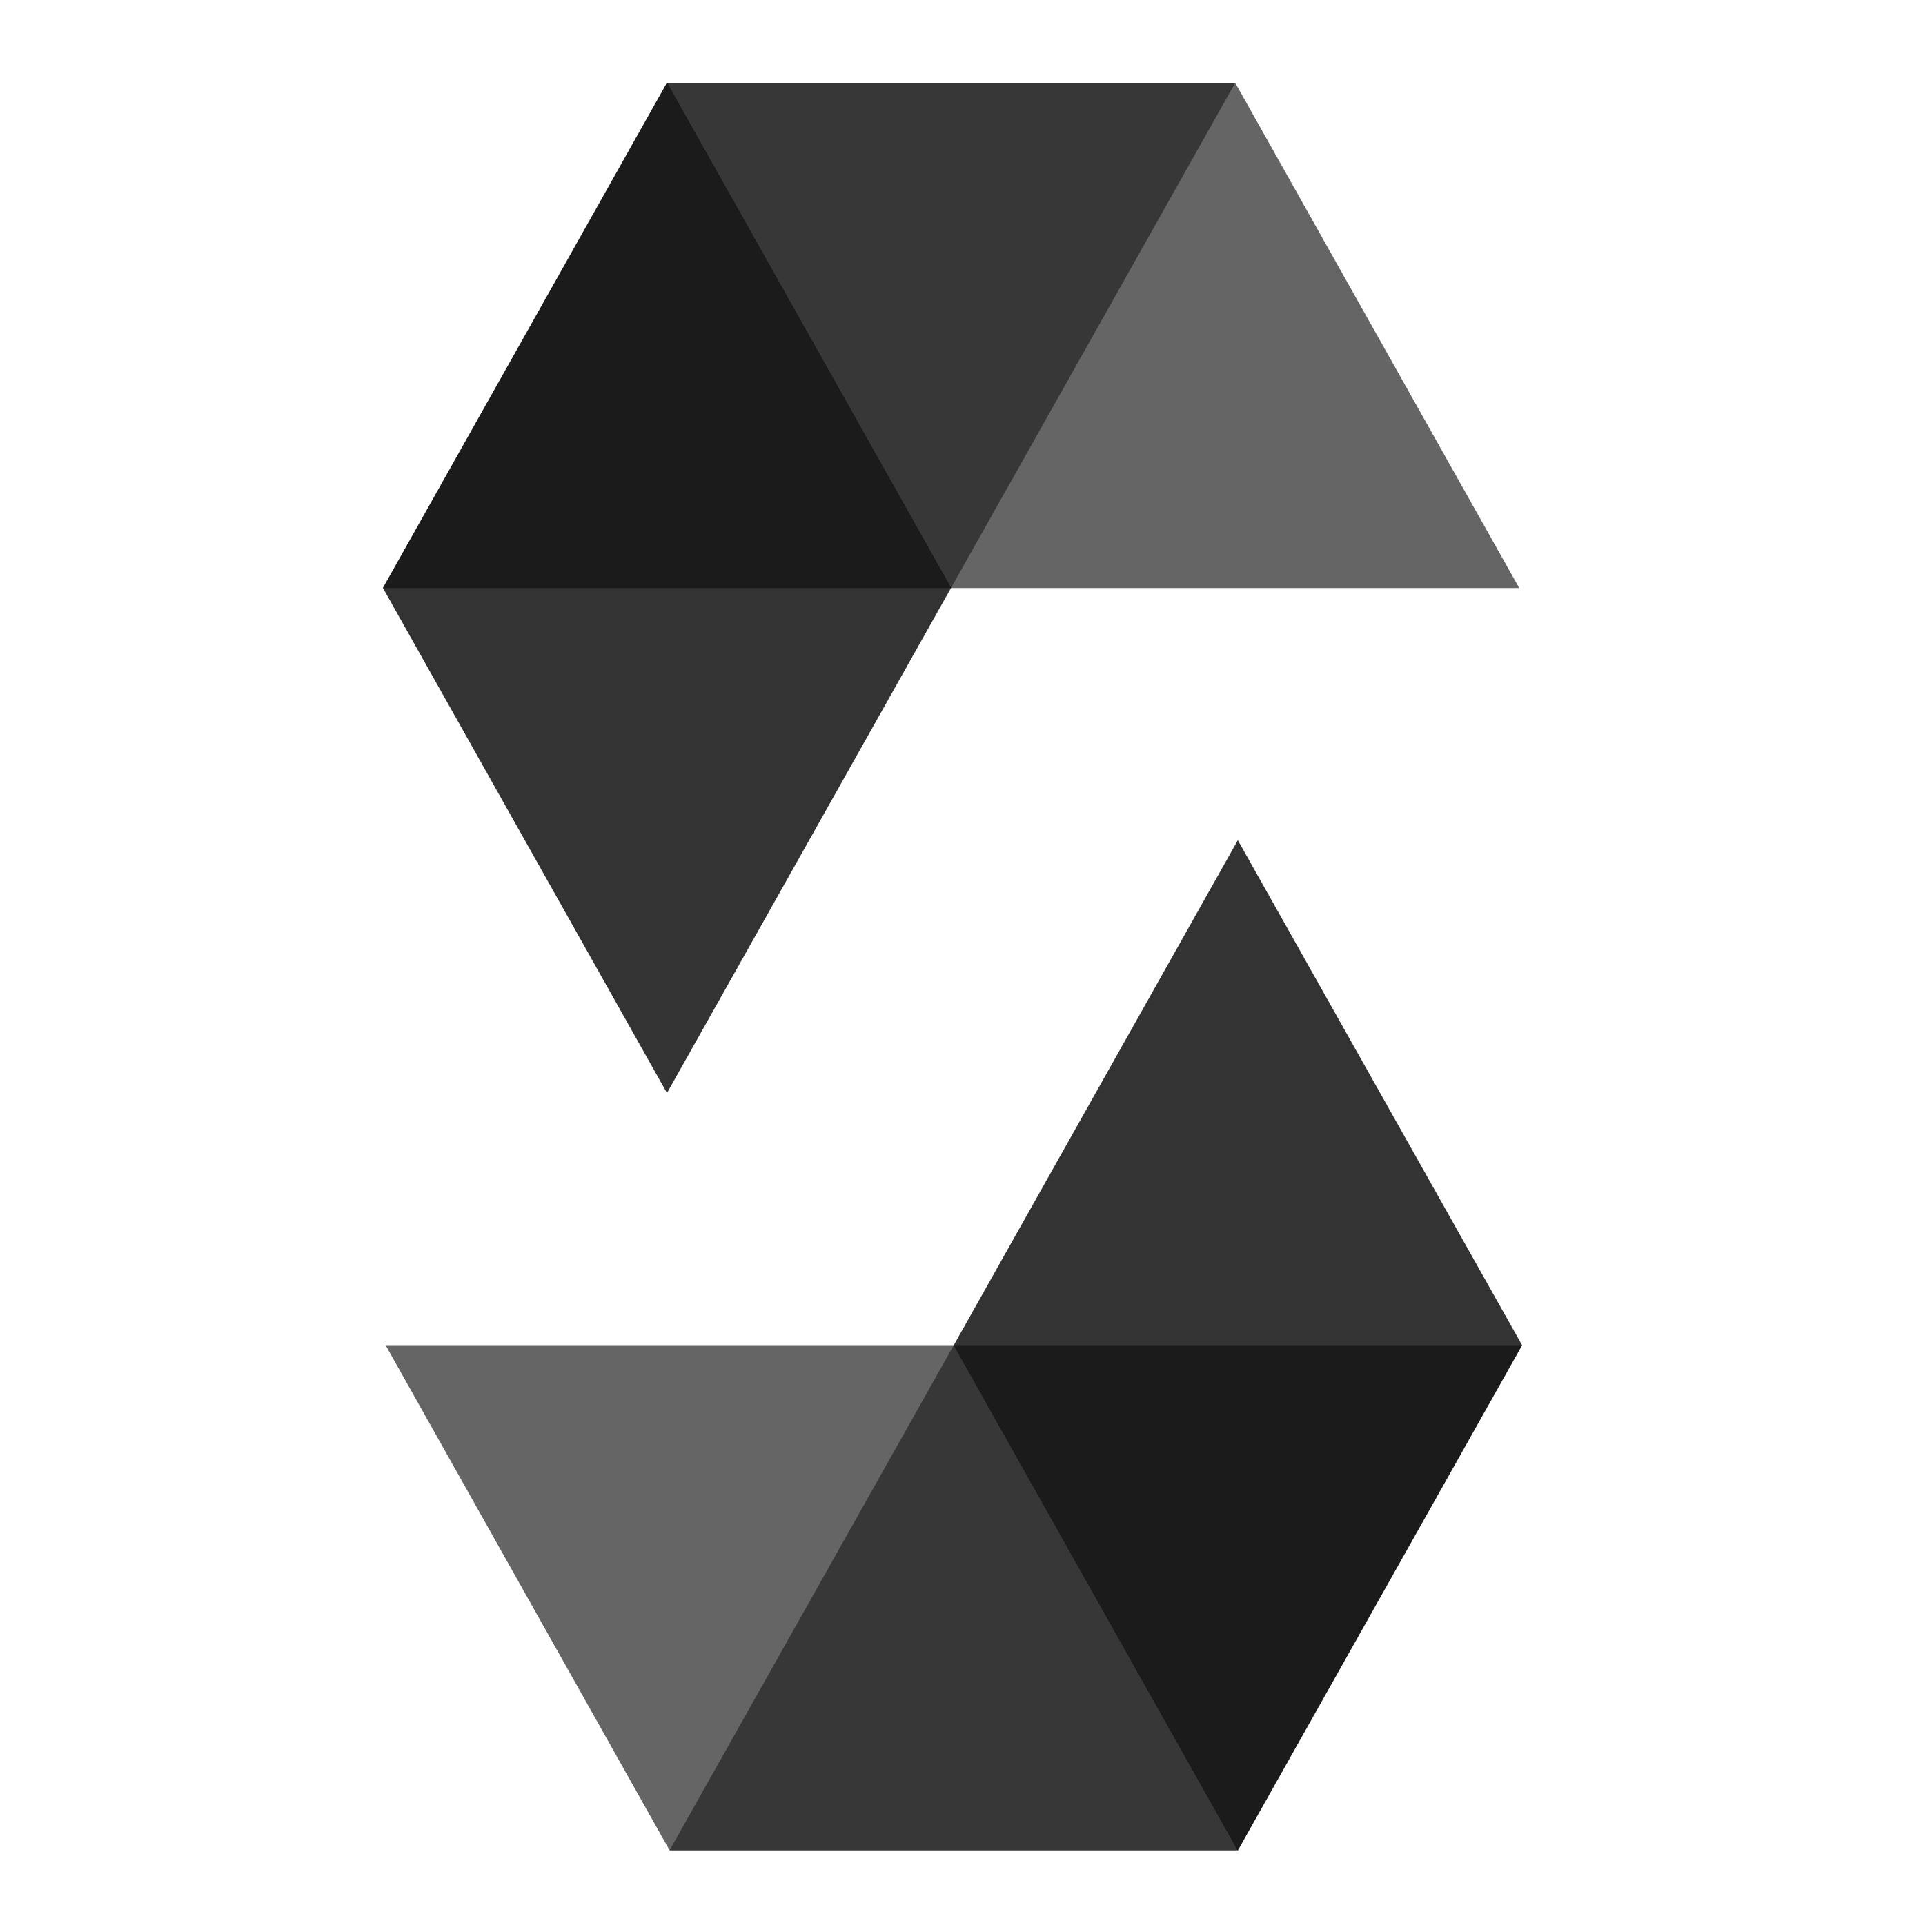
\includegraphics[width=0.2\textwidth]{capitolo3/solidity-logo.png}
%   \caption{Logo di Solidity}
%   \textbf{Fonte}: \href{https://docs.soliditylang.org/en/v0.8.6}{https://docs.soliditylang.org}
% \end{figure}

\noindent Alcuni costrutti di Solidity degni di nota sono:
\begin{itemize}
  \item \textbf{non esiste il \textit{null}} e tutte le variabili, se non assegnate in fase di creazione, avranno un valore di \textit{default} in base al loro tipo;
  \item le funzioni che non modificano lo stato dello \textit{smart contract} possono essere contrassegnate come \textbf{\textit{view}} e non verrà speso del \textit{Gas} per eseguirle;
  \item la presenza di \textbf{modificatori}, ovvero funzioni che eseguono del codice prima, o dopo, una funzione. Vengono per lo più utilizzati per la dichiarazione di condizioni d'esecuzione di una funzione, cioè se non rispetta una regola non può essere eseguita. Riducono di molto le ripetizioni di codice e permettono l'implementazione di vari \textit{design pattern}; 
  \item possono essere dichiarati e lanciati \textbf{eventi} che segnalano al mondo esterno allo \textit{smart contract} l'avvenimento di qualcosa;
  \item la presenza della funzione \textit{built-in} chiamata \textbf{\textit{require}}, la quale permette di far fallire l'esecuzione dello \textit{smart contract} se non viene rispettata una determinata condizione.
\end{itemize}

\paragraph{Tipi di transazioni}
Grazie all'introduzione degli \textit{smart contract} vengono ampliate le tipologie di transazione che si possono eseguire. Viene anche introdotto il concetto di EOA (\textit{Externally Owned Accounts}), il quale rappresenta qualsiasi elemento che nella \textit{blockchain} Ethereum può ricevere o inviare soldi (anche uno \textit{smart contract}). \\

\noindent I tipi di transazioni sono i seguenti:
\begin{itemize}
  \item \textbf{Scambio di moneta}: questo è l'unico tipo di transazione dove il destinatario può essere anche un \textit{wallet}. Nel caso in cui sia un \textit{wallet} allora verranno inviati i soldi. Nel caso in cui, invece, il EOA sia un contratto, verrà incrementato il bilancio interno allo \textit{smart contract} invocando un metodo di tipo \textit{payable} oppure utilizzando quello di \textit{fallback};
  
  \begin{figure}[h!]
    \centering
    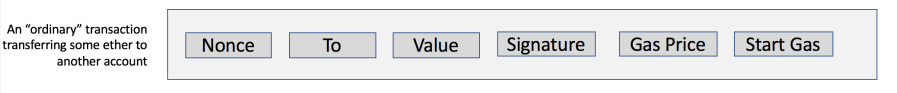
\includegraphics[width=\textwidth]{capitolo3/studio-preliminare/ethereum-transaction-send-money.png}
    \caption{Transazione di scambio di moneta in Ethereum}
    \textbf{Fonte}: \href{https://github.com/spoto/blockchain-course/tree/master/Ethereum}{https://github.com/spoto/blockchain-course/tree/master/Ethereum} 
  \end{figure}

  \item \textbf{Creazione di un contratto}: consiste in una transazione dove viene eseguita l'installazione di un contratto all'interno di un blocco. In questo caso il campo \textit{to} verrà impostato con valore 0. In seguito all'installazione verrà ritornato l'indirizzo del blocco dove è presente lo \textit{smart contract};
  
  \begin{figure}[h!]
    \centering
    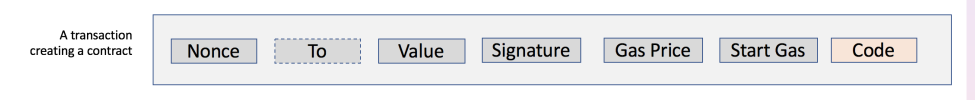
\includegraphics[width=\textwidth]{capitolo3/studio-preliminare/ethereum-transaction-create-contract.png}
    \caption{Transazione di creazione di un nuovo contratto in Ethereum}
    \textbf{Fonte}: \href{https://github.com/spoto/blockchain-course/tree/master/Ethereum}{https://github.com/spoto/blockchain-course/tree/master/Ethereum} 
  \end{figure}
  
  \item \textbf{Invocazione di un contratto}: consiste in una transazione dove viene invocato un metodo presente in uno \textit{smart contract} precedentemente installato. In questo caso il campo \textit{to} corrisponderà all'indirizzo dello \textit{smart contract} interessato e il campo \textit{data} il metodo da invocare.
  
  \begin{figure}[h!]
    \centering
    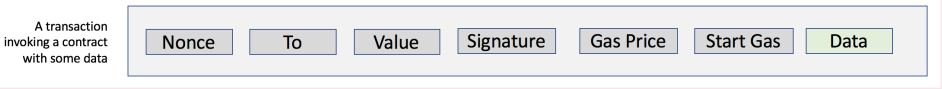
\includegraphics[width=\textwidth]{capitolo3/studio-preliminare/ethereum-transaction-invoke-contract.png}
    \caption{Transazione di invocazione di un contratto in Ethereum}
    \textbf{Fonte}: \href{https://github.com/spoto/blockchain-course/tree/master/Ethereum}{https://github.com/spoto/blockchain-course/tree/master/Ethereum} 
  \end{figure}
\end{itemize}

\paragraph{Lo stato di Ethereum}
Lo stato in Ethereum è molto complesso e si affida ad una struttura dati chiamata \textit{\textbf{Merkle PATRICIA tries}}, in quanto delle semplice mappe chiave valore non possono permettere il \textit{checkout} delle operazioni. Infatti, la principale necessità dello stato di Ethereum è la possibilità di eseguire l'operazione di \textit{checkout} tornando indietro ad un determinato stato ed eseguire di nuovo tutte le operazioni successive. Questa necessità deriva dal fatto che, in caso di diramazioni dello stato non è possibile ignorarle come fa BitCoin, perché trattandosi di operazioni bisogna allineare lo stato rieseguendole. \\

Il \textbf{\textit{PATRICIA Trie}} è un albero che permette di conservare una serie di dati di tipo chiave valore e poi di recuperarli in modo semplice ed efficiente. La chiave indica il percorso da seguire per giungere alla foglia che contiene il valore corrispondente. Nel caso di Ethereum, il \textit{PATRICIA Trie} viene modificato con concetti visti nel \textit{Merkle Tree}, come ad esempio il fatto che il puntatore ad un nodo sia il hash crittografico del nodo stesso.

%%%%%%%%%%%%%%%%%%%%%%%%%%%%%%%%%%%%%%%%%%%%%%%%%%%%%%%%%%%%%%%%%%%%%%%%%%%%%%%%%%%

\subsection{La blockchain Hotmoka}
Hotmoka è un \textit{framework} per la programmazione di una rete \textit{peer-to-peer}, attraverso un sottoinsieme di Java chiamato Takamaka. I nodi possono appartenere a una \textit{blockchain} o possono essere dispositivi IOT (\textit{Internet Of Things}). È sviluppata e mantenuta dall'Università degli Studi di Verona.

% \begin{figure}[h!]
%   \centering
%   
\includegraphics[width=0.4\textwidth]{capitolo3/hotmoka-logo.png}
%   \caption{Logo di Hotmoka}
%   \textbf{Fonte}: \href{https://hotmoka.io}{https://hotmoka.io}
% \end{figure}

\paragraph{Cos'è Tendermint}
Tendermint è un \textit{framework} per la scrittura di \textit{blockchain}. Infatti, come si può vedere in figura \ref{fig:tendermint-structure}, il \textit{core} di Tendermint ha solo il compito di gestire i blocchi della \textit{blockchain} e comunicare con gli altri \textit{peer} di essa. Lo stato della \textit{blockchain} consisterà solo nel hash della transazione. Ciò che viene demandato al programmatore è lo sviluppo del \textit{application layer}, ovvero la definizione di tutto quello che viene memorizzato nella \textit{blockchain}. Per comunicare con il Tendermint \textit{core} e rendere tutto il più possibile indipendentemente dall'implementazione, l'\textit{application layer} definisce solamente una serie di funzioni che verranno richiamate durante il salvataggio di un blocco da parte del \textit{core} attraverso \textit{sockets}. \\

\noindent Le funzioni da implementare nel \textit{application layer} sono le seguenti:
\begin{itemize}
  \item \textbf{\textit{checkTX}}: ha il compito di filtro per le transazioni in ingresso, controllando la loro forma sintatticamente corretta;
  \item \textbf{\textit{beginBlock}}: chiamata all'inizio del blocco, riceve informazioni circa l'insieme dei validatori e quali hanno firmato il blocco precedente;
  \item \textbf{\textit{deliverTX}}: viene chiamata per ogni transazioni e modifica lo stato dell'\textit{application layer};
  \item \textbf{\textit{endBlock}}: viene chiamata alla fine del blocco fornendo informazioni circa l'insieme dei validatori per il prossimo blocco;
  \item \textbf{\textit{commit}}: viene chiamata quando il blocco è stato aggiunto e fornisce il hash dello stato dell'\textit{application layer};
  \item \textbf{\textit{query}}: chiamata per la lettura di dati su \textit{blockchain}.
\end{itemize}

\begin{figure}[h!]
  \centering
  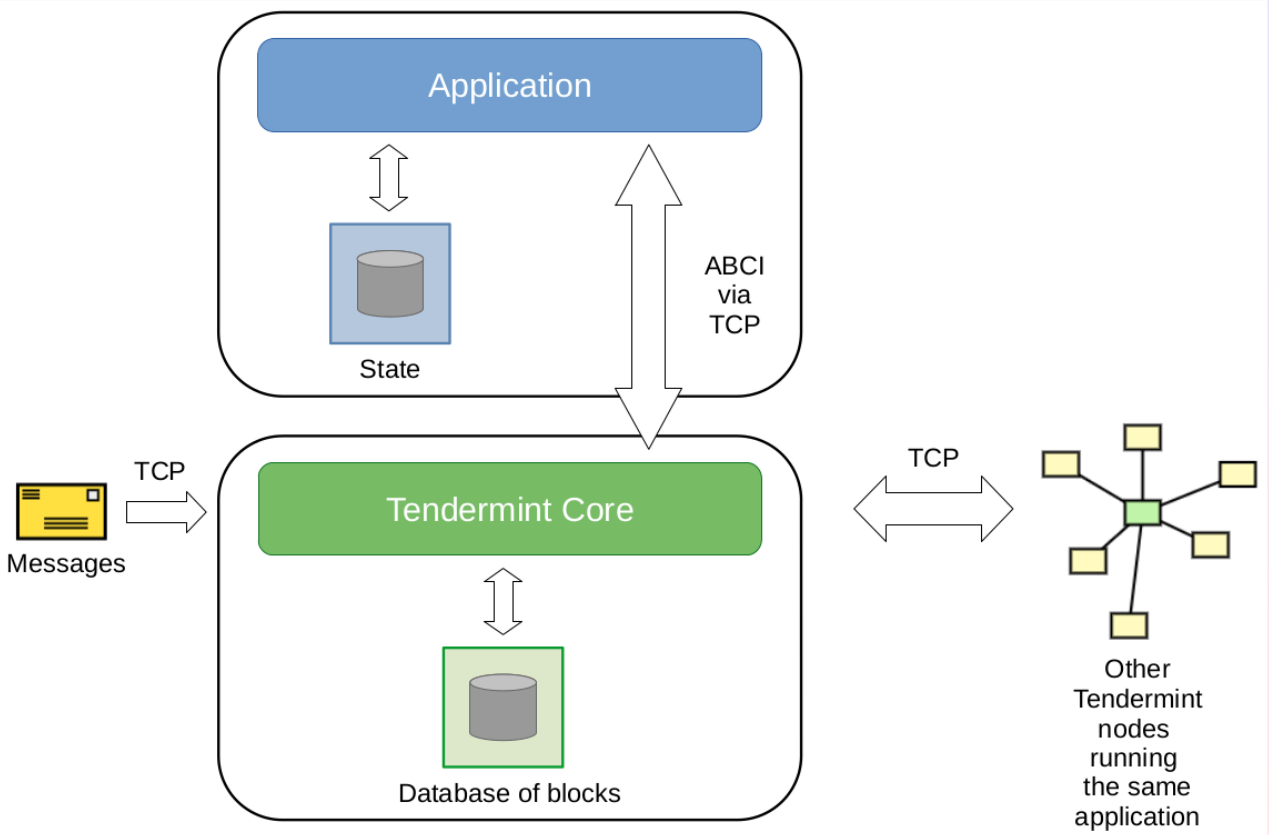
\includegraphics[width=0.8\textwidth]{capitolo3/studio-preliminare/tendermint-structure.png}
  \caption{Struttura di Tendermint}
  \textbf{Fonte}: \href{https://github.com/spoto/blockchain-course/tree/master/Tendermint}{https://github.com/spoto/blockchain-course/tree/master/Tendermint} 
  \label{fig:tendermint-structure}
\end{figure}

Un'altra caratteristica molto importante per quanto riguarda Tendermint è l'utilizzo dell'algoritmo del consenso \textit{Proof of Stake}, piuttosto del troppo lento e impegnativo \textit{Proof of Work}.
\textbf{\textit{Proof of Stake}} è una variante del \gls{Practical Byzantine Fault Tolerance}, dove viene raggiunto il consenso attraverso i nodi che si comportano in maniera corretta. In \textit{Proof of Stake} ci si basa sulla quantità di \textit{stake}, ovvero moneta, che un determinato \textit{peer} possiede. \\

\noindent I passi dell'algoritmo \textit{Proof of Stake} sono i seguenti:
\begin{enumerate}[label=\lett]
  \item un insieme dinamico \( V \) di validatori decidono un prossimo nodo in base alla quantità di \textit{stake} che possiede. L'insieme \( V \) sarà diverso per ogni nodo e viene deciso in base all'esecuzione che è avvenuta precedentemente;
  \item ogni validatore \( v \in V \) a questo punto:
  \begin{enumerate}[label=\arabic*.]
    \item identifica deterministicamente un validatore \( p \in V \), per il quale si aspetta che dovrebbe aggreggare alcune transazioni e proporre un blocco successivo \( b \). In particolare il seguente \textit{peer} riceverà l'approvazione di prendere delle transazioni dalla \textit{mempool} e creare il blocco;
    \item se il blocco \( b \) che è stato generato è considerato valido, allora si pre vota \( b \);
    \item si contano quanti validatori pre votano \( b \);
    \item se almeno \( \frac{2}{3} \) della rete pre votano \( b \), allora si pre invia il blocco \( b \);
    \item si contano quanti validatori pre inviano \( b \);
    \item se almeno \( \frac{2}{3} \) della rete pre inviano il blocco \( b \), allora \( b \) viene inviato;
    \item si torna al punto \textbf{a}.
  \end{enumerate}
\end{enumerate}

\clearpage
\begin{figure}[h!]
  \centering
  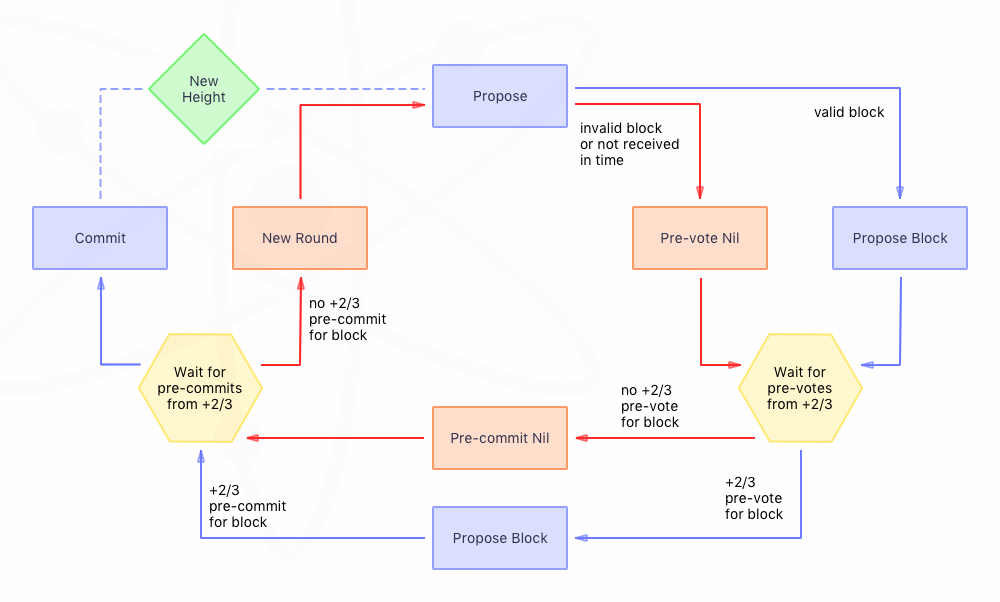
\includegraphics[width=0.9\textwidth]{capitolo3/studio-preliminare/tendermint-pos.png}
  \caption{Esecuzione di \textit{Proof of Stake} in Tendermint}
  \textbf{Fonte}: \href{https://blog.cosmos.network/consensus-compare-casper-vs-tendermint-6df154ad56ae}{https://blog.cosmos.network/consensus-compare-casper-vs-tendermint}
\end{figure}

\noindent Tendermint è stato utilizzato per la realizzazione di Hotmoka.

\paragraph{Gli smart contract in Hotmoka}
Gli \textit{smart contract} in Hotmoka sono programmabili attraverso un \textit{subset} di Java chiamato Takamaka. \textbf{Takamaka} aggiunge molte annotazioni e classi per facilitare la scrittura di \textit{smart contract}, andando ad imitare i costrutti degni di nota del linguaggio Solidity che ho elencato in §\ref{par:ethereum.smart-contract}. Inoltre viene rimosso l'accesso a tutti i costrutti di programmazione concorrente e alle funzioni che potrebbero creare non determinismo. Viene introdotto, come per Ethereum, il concetto di \textit{Gas price} e \textit{Gas limit}. \\

Ogni \textit{smart contract} verrà pacchettizzato come \textbf{JAR} e, dopo aver eseguito un processo di verifica, dove verrà controllato che tutte le istruzioni scritte siano consentite, e di instrumentizzazione, dove verrà modificato e reso installabile dentro un blocco, viene inviato alla rete Hotmoka.  
Il pacchetto JAR a questo punto sarà installato all'interno di essa e potrà essere richiamabile da altri \textit{smart contract}.
In seguito potranno essere istanziati oggetti di quello \textit{smart contract} sul quale invocare tutte le funzioni disponibili.

% \begin{figure}[h!]
%   \centering
%   
\includegraphics[width=0.4\textwidth]{capitolo3/takamaka-logo.png}
%   \caption{Logo di Takamaka}
%   \textbf{Fonte}: \href{https://www.takamaka.io}{https://www.takamaka.io}
% \end{figure}

\paragraph{Lo stato di Hotmoka}
Essendo un'implementazione di Tendermint, Hotmoka presenta sia lo stato della \textit{blockchain}, gestito da Tendermint \textit{core}, e sia lo stato del \textit{application layer}. Quest'ultimo deve memorizzare due categorie di dato: i JAR che vengono inviati e gli oggetti istanziati. \\

Dato che il salvataggio dei JAR e degli oggetti deve essere persistente, è stata data una struttura ben definita allo stato, il quale è stato diviso in: \textit{reponses} e \textit{histories}.

Lo stato \textbf{\textit{responses}} ha il compito di memorizzare la risposta di ogni transazione che è stata effettuata. Associa il hash della transazione (\textit{request}) effettuata ad una determinata risposta. 
La risposta può essere di due tipi:
\begin{itemize}
  \item \textbf{JAR}: se la richiesta a cui è associata corrisponde alla memorizzazione di un JAR. In questo caso dentro la risposta verrà memorizzato il JAR che è stato inserito in un blocco;
  \item \textbf{Field updates}: se la richiesta a cui è associata corrisponde alla creazione di un oggetto oppure all'invocazione di metodi che modificano lo stato. In questo caso la risposta conterrà o l'oggetto istanziato, oppure il valore dei campi che sono stati aggiornati dall'invocazione di un metodo.
\end{itemize}

\begin{figure}[h!]
  \centering
  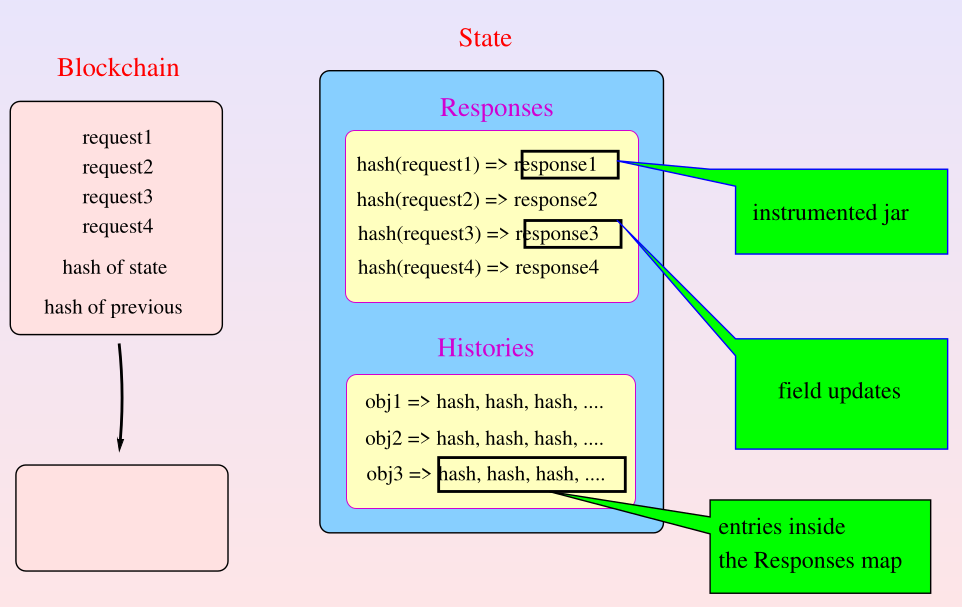
\includegraphics[width=0.8\textwidth]{capitolo3/studio-preliminare/hotmoka-state.png}
  \caption{Lo stato di un blocco nella \textit{blockchain} Hotmoka}
  \textbf{Fonte}: \href{https://github.com/spoto/blockchain-course/tree/master/Hotmoka}{https://github.com/spoto/blockchain-course/tree/master/Hotmoka}
\end{figure}

L'implementazione tipica di questo stato viene data attraverso l'utilizzo di un \textbf{\textit{Merkle Tree}}, la quale \textit{Merkle root} viene memorizzata dentro il blocco che deve essere salvato in \textit{blockchain}. \\

Lo stato \textbf{\textit{histories}}, invece, viene utilizzato per associare ad ogni oggetto il hash delle risposte che per ultime hanno modificato un suo attributo, in modo tale da poter ricostruire il suo stato. Da questo ne consegue che se un oggetto ha 3 campi, la sua storia potrà essere lunga al massimo 3, visto che si terrà sempre l'ultima richiesta che ha modificato un attributo.

%%%%%%%%%%%%%%%%%%%%%%%%%%%%%%%%%%%%%%%%%%%%%%%%%%%%%%%%%%%%%%%%%%%%%%%%%%%%%%%%%%%

\subsection{Lo standard ERC721}
Per ERC (\textit{Ethereum Request Comments}) si intendono le richieste di standardizzazione che avvengono nella \textit{blockchain} Ethereum per la scrittura di \textit{smart contract}. Sono associate ad un numero progressivo e quella che gestisce gli \textbf{NFT} è stata la numero 721. \\

% \clearpage
% \begin{figure}[h!]
%   \centering
%   
\includegraphics[width=0.3\textwidth]{capitolo3/open-zeppelin-logo.png}
%   \caption{Logo dell'azienda OpenZeppelin}
%   \textbf{Fonte}: \href{https://openzeppelin.com/}{https://openzeppelin.com/}
% \end{figure}

Per lo sviluppo dello \textit{smart contract} in \textbf{Solidity} è stata utilizzata l'implementazione dello standard ERC721 più utilizzata e conosciuta nel mondo Ethereum, ovvero quella data dall'azienda \textbf{OpenZeppelin}. Oltre alla sua grande fama e al fatto che è utilizzata dalla maggior parte della \textit{community}, è stata scelta perché non ci sono vulnerabilità attualmente conosciute. \\

Per quanto riguarda invece \textbf{Hotmoka}, essendo una \textit{blockchain} giovane non è stato implementato alcuno standard per la scrittura di \textit{smart contract} per la gestione di NFT. Per questo motivo, in accordo con il mio \textit{tutor} aziendale, Fabio Pallaro, è stato deciso che avrei provato a scrivere una mia possibile implementazione dello standard ERC721.

%%%%%%%%%%%%%%%%%%%%%%%%%%%%%%%%%%%%%%%%%%%%%%%%%%%%%%%%%%%%%%%%%%%%%%%%%%%%%%%%%%%

\subsection{Il protocollo IPFS (InterPlanetary File System)}
Il protocollo IPFS (\textit{InterPlanetary File System}) è un'alternativa al protocollo internet HTTP. IPFS si pone l'obiettivo di creare una rete informatica di portata globale che consenta l'archiviazione delle informazioni in maniera completamente decentralizzata e con elevata scalabilità. \\

% \begin{figure}[h!]
%   \centering
%   
\includegraphics[width=0.2\textwidth]{capitolo3/ipfs-logo.png}
%   \caption{Logo di IPFS}
%   \textbf{Fonte}: \href{https://ipfs.io}{https://ipfs.io}
% \end{figure}

È attualmente la risposta tecnologica ai limiti di HTTP che ad oggi sembra più concreta. Il protocollo infatti promette di sostituire HTTP, adottando come base tecnica e concettuale un modello di decentralizzazione dei contenuti. Il web di oggi è inefficiente e costoso, dove HTTP permette di scaricare \textit{file} da un computer alla volta invece di ottenere parti degli stessi da più computer contemporaneamente. In più fa riferimento ai \textit{file} attraverso la \textbf{\textit{location addressing}}, cioè attraverso il nome con il quale vengono riconosciuti dal \textit{File System}. Questo può comportare vari problemi nell'ambito degli NFT, infatti se un \textit{hacker} o una qualsiasi altra persona cambiasse un'opera a cui è associato un NFT con un'altra, ma mantenendo lo stesso nome del \textit{file}, il sistema non si accorgerebbe di nulla e si perderebbe così l'opera vera e propria, causando un'incongruenza nei dati. 
Uno dei punti di forza di IPFS è proprio il non utilizzare la \textit{location addressing}, ma bensì il \textbf{\textit{content addressing}}. Tramite questo metodo di indirizzamento, ogni file viene associato ad un codice univoco, chiamato \textbf{CID (\textit{Content ID})}, che si basa sul contenuto del \textit{file}. In questo modo ogni \textit{file} potrà essere riferito attraverso il proprio CID e non potrà essere sostituito in alcun modo da altri, visto che avranno un CID diverso.
Oltre a questo motivo, è stato scelto di utilizzare IPFS anche per la sua natura decentralizzata che assicura sempre la reperibilità delle opere richieste. \\

% Ogni nodo memorizza la rete attraverso una struttura dati chiamata \textit{Merkle DAG (Directed Acyclic Graph)}, dove ogni nodo ha un identificativo ottenuto dall'operazione di \textit{hashing} dei contenuti di esso, ovvero i \text{file} contenuti, attraverso una funzione crittografica come può essere SHA256.

% Per quanto concerne il funzionamento e la comunicazione tra i vari nodi della rete, viene utilizzato il protocollo \textbf{\textit{BitSwap}}, ovvero un protocollo per lo scambio di blocchi di dati simile a \textit{BitTorrent}.
% Questo protocollo dirige e gestisce la richiesta e l'invio di blocchi da e verso altri \textit{peer} nella rete. \textit{BitSwap} ha due compiti principali: 
% \begin{itemize}
%   \item acquisire i blocchi richiesti dal client dalla rete;
%   \item inviare i blocchi in suo possesso ad altri peer che lo desiderano.
% \end{itemize}

% IPFS suddivide i \textit{file} in blocchi di dati, identificando ognuno di essi attraverso un CID. Quando qualcuno esegue la richiesta di un \textit{file}, comunica con un nodo della rete il quale, se ha salvato il proprio file glielo invia, altrimenti inizia l'operazione di \textit{discovery}. Qui entra in gioco il protocollo \textit{BitSwap}, il quale prima di tutto invia una richiesta a tutti i \textit{peer} con il quale è connesso dove chiede chi ha il CID di un blocco o direttamente di tutto il \textit{file}. I \textit{peer} vicini gli risponderanno di si se ce l'hanno e no chi non ce l'ha. Questi ultimi comunicheranno con quelli vicini e faranno la stessa domanda, fino a quando la richiesta non passa per un certo numero di \textit{peer} e non viene più inviata. Invece al primo \textit{peer} che ha risposto che ha quel CID, viene fatta la richiesta di inviarglielo. Dopo averlo ricevuto, invia una richiesta di cancellazione della richiesta, in modo tale da non dover far propagare la richiesta del blocco nella rete.

% \clearpage

% \begin{figure}[h!]
%   \centering
%   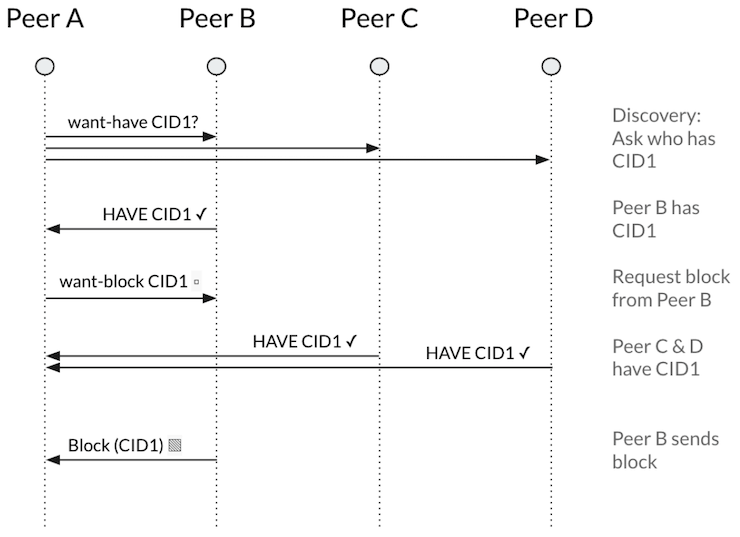
\includegraphics[width=0.8\textwidth]{capitolo3/ipfs-bitswap.png}
%   \caption{Esempio di esecuzione del protocllo \textit{BitSwap}}
%   \textbf{Fonte}: \href{https://docs.ipfs.io/concepts/bitswap}{https://docs.ipfs.io/concepts/bitswap}
% \end{figure}

Essendo IPFS un protocollo a se stante rispetto a HTTP, per poterlo utilizzare in NFTLab c'erano due strade da poter intraprendere:
\begin{enumerate}
  \item utilizzare un nodo IPFS locale per connettersi alla rete;
  \item utilizzare un servizio online per la comunicazione con la rete IPFS.
\end{enumerate}

La prima proposta è stata scartata subito perché avrebbe solamente complicato ancora di più il sistema che dovevo tenere in piedi per lo sviluppo. Per questo è stata intrapresa la seconda strada e, in seguito ad una ricerca di quale fosse il servizio più conveniente, è stato scelto \textbf{Pinata} visto che è il più famoso in circolazione e  offre delle comode \gls{api} da richiamare per caricare e prelevare \textit{file} dalla rete IPFS.

\clearpage
\begin{figure}[h!]
  \centering
  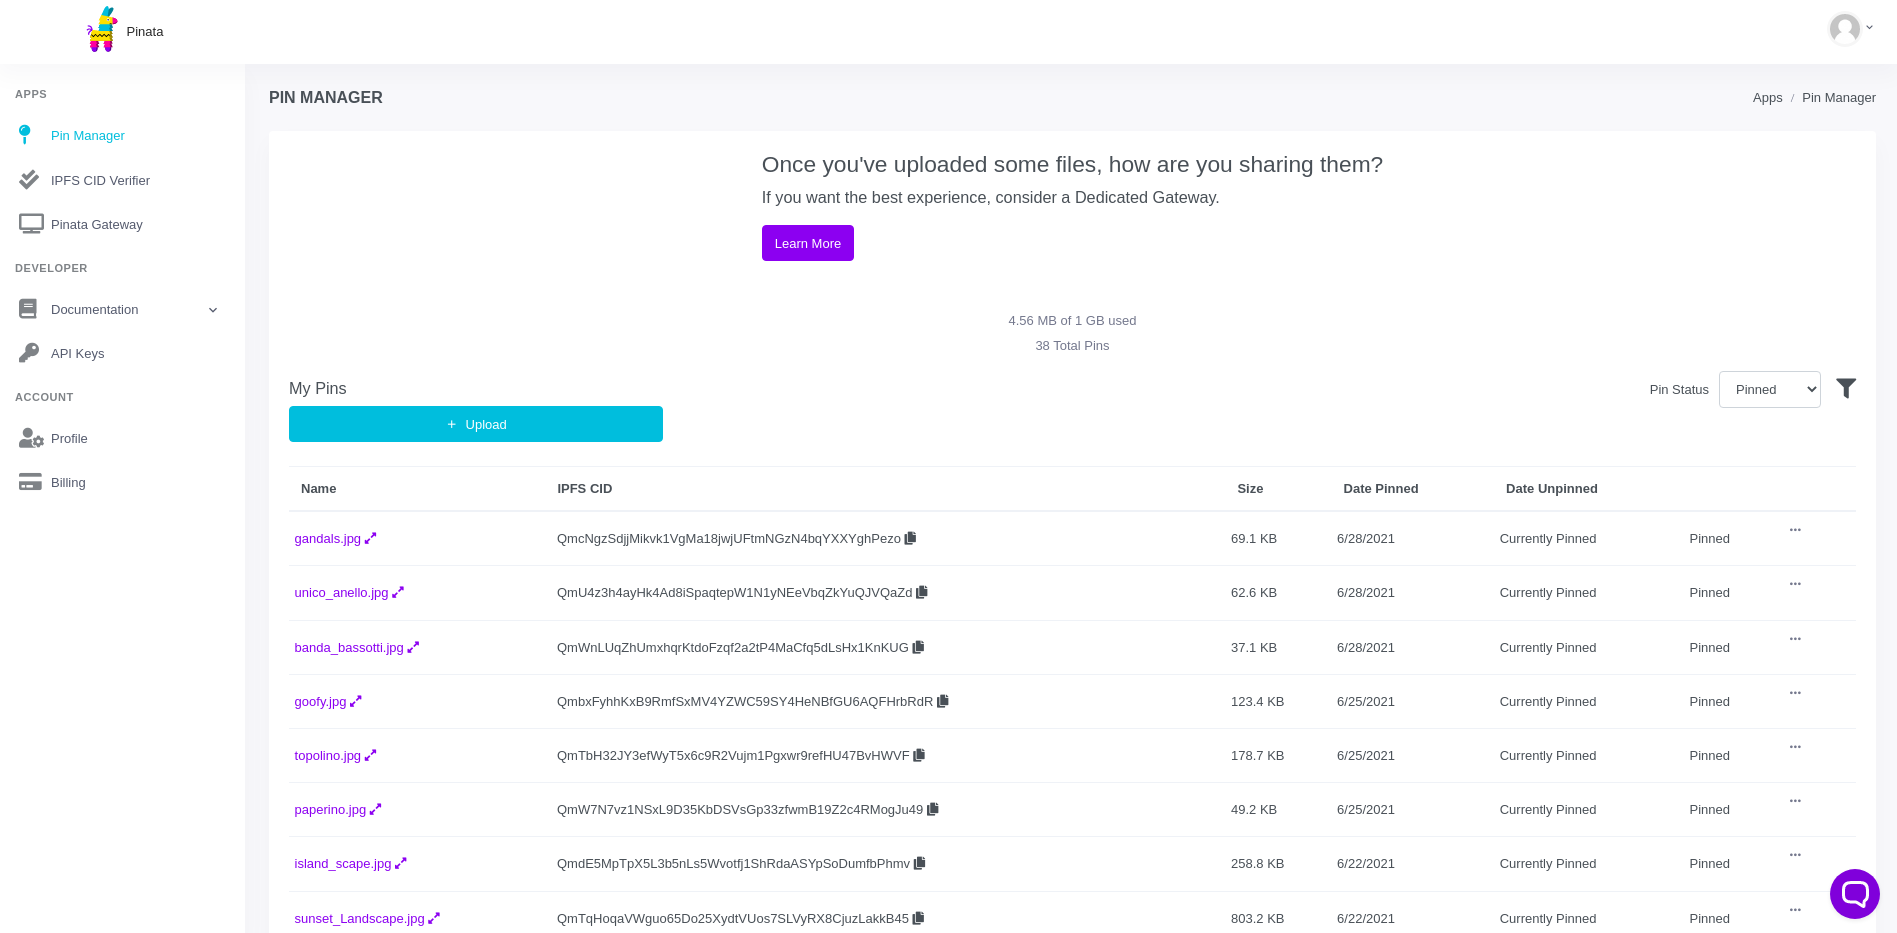
\includegraphics[width=\textwidth]{capitolo3/ipfs-pinata-dashboard.png}
  \caption{\textit{Dashboard} personale di Pinata}
\end{figure}


%%%%%%%%%%%%%%%%%%%%%%%%%%%%%%%%%%%%%%%%%%%%%%%%%%%%%%%%%%%%%%%%%%%%%%%%%%%%%%%%%

% !TEX encoding = UTF-8
% !TEX TS-program = pdflatex
% !TEX root = ../tesi.tex


%%%%%%%%%%%%%%%%%%%%%%%%%%%%%%%%%%%%%%%%%%%%%%%%%%%%%%%%%%%%%%%%%%%%%%%%%%%%%%%%%

% !TEX encoding = UTF-8
% !TEX TS-program = pdflatex
% !TEX root = ../../tesi.tex

\section{Analisi dei requisiti}
Ho iniziato la fase di analisi dei requisiti dalla quarta settimana di lavoro, cioè quando, come pianificato, avrei dovuto iniziare ad implementare gli \textit{smart contract} per la gestione di NFT seguendo gli standard ERC su \textit{blockchain} Ethereum. Inizialmente è avvenuto un processo di \textit{brainstorming} con gli altri componenti del gruppo e i vari \textit{tutor} di ognuno di noi per definire al meglio le funzionalità della piattaforma. In seguito ho isolato e ridotto le funzionalità ed i requisiti che avrebbe dovuto la mia libreria e lo \textit{smart contract} che avrei dovuto implementare. Per quanto riguarda i casi d'uso, vengono utilizzati i diagrammi dei casi d'uso per facilitarne la Presentazione concettuale, mentre per i requisiti sono state utilizzate delle tabelle di tracciamento. 

\subsection{Casi d'uso}
I casi d'uso sono una tecnica utilizzata nel processo di analisi dei requisiti per effettuare in maniera esaustiva e non ambigua, la raccolta dei requisiti al fine di produrre \textit{software} di qualità. \\

\noindent La classificazione dei casi d'uso ha seguito la seguente convenzione:
\begin{center}
  UC[NumeroCasoBase](.[NumeroSottoCaso])*
\end{center}
dove:
\begin{itemize}
  \item \textbf{NumeroCasoBase}: è costituito da un numero progressivo che indica il caso d'uso generico;
  \item \textbf{NumeroSottoCaso}: è costituito da un numero progressivo opzionale che indica il sotto-caso d'uso del caso
  d'uso generico.
\end{itemize}

\subsubsection{Attori primari}
Un attore primario è colui che interagisce con il sistema per un determinato scopo.
Gli attori primari identificati sono i seguenti:

\begin{figure}[h!]
  \centering
  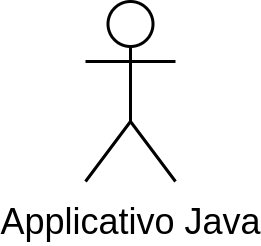
\includegraphics{capitolo3/casi-uso/attori-primari.png}
  \caption{Attori primari}
\end{figure}

\begin{itemize}
  \item \textbf{Applicativo Java}: rappresenta qualsiasi applicazione sviluppata in Java che interagisce con la libreria. In questo caso, consiste nel \textit{back-end} sviluppato utilizzando il \textit{framework} Spring.
\end{itemize}

\subsubsection{Attori secondari}
Un attore secondario è un'entità estranea al sistema che supporta gli attori primari nelle loro attività.

\begin{figure}[h!]
  \centering
  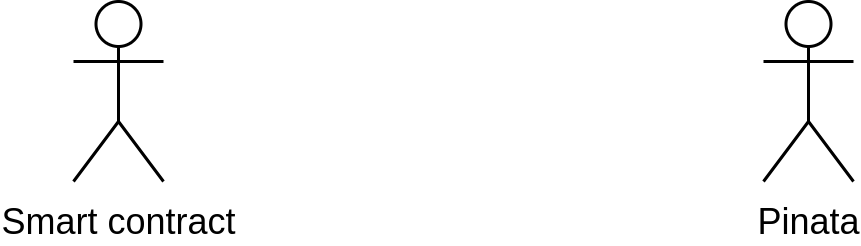
\includegraphics{capitolo3/casi-uso/attori-secondari.png}
  \caption{Attori secondari}
\end{figure}

\begin{itemize}
  \item \textbf{\textit{Smart contract}}: rappresenta lo \textit{smart contract} caricato in \textit{blockchain} con il quale comunicare;
  \item \textbf{Pinata}: rappresenta il servizio che permette di interagire con la rete IPFS.
\end{itemize}

\UC{Caricamento di un opera in blockchain}
Qualsiasi applicativo Java può caricare un opera in blockchain.

\begin{itemize}
  \item \UCPrimaryActors{applicativo Java};
  \item \UCSecondaryActors{\textit{smart contract}, Pinata};
  \item \UCPre{l'applicativo Java vuole creare un NFT da un opera non ancora esistente};
  \item \UCPost{il NFT è stato creato e l'opera è stata caricata nella rete IPFS};
  \item \UCMain
  \begin{itemize}
    \item L'applicativo Java vuole creare un NFT a partire da un opera, dalla quale non è stato creato alcun NFT;
    \item L'opera viene caricata sulla rete IPFS tramite il servizio Pinata;
    \item Viene invocato lo \textit{smart contract} e creato il NFT.
  \end{itemize}
  \item \UCExt
  \begin{enumerate}[label=\lett]
    \item L'applicativo Java vuole assegnare il NFT ad un \textit{wallet} che non è nel formato corretto:
    \begin{itemize}
      \item (UC\ref{UC:extension.wallet-not-correct}) - Visualizzazione messaggio di \textit{wallet} non nel formato corretto;
      \item Viene impedita la creazione del NFT.
    \end{itemize}

    \item L'applicativo Java vuole comunicare con lo \textit{smart contract} attraverso un \textit{wallet}, il quale non è il proprietario di quest'ultimo:
    \begin{itemize}
      \item (UC\ref{UC:extension.operation-not-allowed}) - Visualizzazione messaggio di operazione non consentita;
      \item Viene impedita la creazione del NFT.
    \end{itemize}

    \item L'applicativo Java vuole caricare un'opera dalla quale è già stato estratto il NFT:
    \begin{itemize}
      \item (UC\ref{UC:extension.nft-exists-yet}) - Visualizzazione messaggio di NFT già esistente;
      \item Viene impedita la creazione del NFT.
    \end{itemize}
  \end{enumerate}
\end{itemize}


\UC{Trasferimento della proprietà di un NFT}
L'applicativo Java può trasferire la proprietà di un NFT dal proprietario ad un acquirente.

\begin{itemize}
  \item \UCPrimaryActors{applicativo Java};
  \item \UCSecondaryActors{\textit{smart contract}};
  \item \UCPre{esiste il NFT che si vuole trasferire e l'acquirente è diverso dal proprietario};
  \item \UCPost{il NFT viene trasferito dal proprietario all'acquirente};
  
  \item \UCMain
  \begin{itemize}
    \item L'applicativo Java, attraverso il \textit{wallet} del proprietario dello \textit{smart contract}, comunica con lo \textit{smart contract} caricato nella \textit{blockchain};
    \item Gli invia i dati del proprietario e dell'acquirente;
    \item Viene eseguito il trasferimento.
  \end{itemize}

  \item \UCExt
  \begin{enumerate}[label=\lett]
    \item L'applicativo Java vuole vuole trasferire il NFT dal proprietario all'acquirente, riferendosi ad uno di questi due attraverso un \textit{wallet} che non è nel formato corretto:
    \begin{itemize}
      \item (UC\ref{UC:extension.wallet-not-correct}) - Visualizzazione messaggio di \textit{wallet} non nel formato corretto;
      \item Viene impedito il trasferimento del NFT.
    \end{itemize}

    \item L'applicativo Java vuole comunicare con lo \textit{smart contract} attraverso un \textit{wallet}, il quale non è il proprietario di quest'ultimo:
    \begin{itemize}
      \item (UC\ref{UC:extension.operation-not-allowed}) - Visualizzazione messaggio di operazione non consentita;
      \item Viene impedito il trasferimento del NFT.
    \end{itemize}

    \item L'acquirente corrisponde al proprietario del NFT:
    \begin{itemize}
      \item Visualizzazione messaggio di operazione non andata a buon fine, dato che l'acquirente non può anche essere il proprietario del NFT;
      \item Viene impedito il trasferimento del NFT.
    \end{itemize}
  \end{enumerate}
\end{itemize}

\UC{Ottenimento di un NFT a partire dal suo id}
L'applicativo Java può ottenere le informazioni di un NFT a partire dal id con il quale è memorizzato.

\begin{itemize}
  \item \UCPrimaryActors{applicativo Java};
  \item \UCSecondaryActors{\textit{smart contract}};
  \item \UCPre{l'applicativo Java utilizza un id associato ad un NFT};
  \item \UCPost{l'applicativo Java ottiene le informazioni del NFT};
  \item \UCMain
  \begin{itemize}
    \item l'applicativo Java invoca lo \textit{smart contract} utilizzando un id associato ad un NFT;
    \item riceve le informazioni inserite durante la creazione.
  \end{itemize}

  \item \UCExt
  \begin{enumerate}[label=\lett]
    \item L'applicativo Java invia un id che non è associato ad alcun NFT:
    \begin{itemize}
      \item (UC\ref{UC:extension.nft-not-exists}) - Visualizzazione messaggio di NFT non esistente;
    \end{itemize}
  \end{enumerate}
\end{itemize}

\UC{Ottenimento di un opera a partire dal suo hash}
L'applicativo Java può ottenere le informazioni di un NFT a partire dal hash associato al NFT.

\begin{itemize}
  \item \UCPrimaryActors{applicativo Java};
  \item \UCSecondaryActors{\textit{smart contract}};
  \item \UCPre{l'applicativo Java utilizza un hash associato ad un NFT};
  \item \UCPost{l'applicativo Java ottiene le informazioni del NFT};
  
  \item \UCMain
  \begin{itemize}
    \item l'applicativo Java invoca lo \textit{smart contract} utilizzando il hash associato al NFT;
    \item riceve le informazioni inserite durante la creazione. 
  \end{itemize}
  
  \item \UCExt
  \begin{enumerate}[label=\lett]
    \item l'applicativo Java invia un hash che non è associato ad alcun NFT:
    \begin{itemize}
      \item (UC\ref{UC:extension.nft-not-exists}) - Visualizzazione messaggio di NFT non esistente.
    \end{itemize}
  \end{enumerate}
\end{itemize}

\UC{Ottenimento della storia delle transazioni di un NFT}
L'applicativo Java può ottenere la storia delle transazioni di un NFT a partire dal id con il quale è memorizzato.

\begin{itemize}
  \item \UCPrimaryActors{applicativo Java};
  \item \UCSecondaryActors{\textit{smart contract}};
  \item \UCPre{l'applicativo Java utilizza un id associato ad un NFT};
  \item \UCPost{L'applicativo Java ottiene la storia delle transazioni di un NFT};

  \item \UCMain
  \begin{itemize}
    \item l'applicativo Java invoca lo \textit{smart contract} utilizzando un id associato ad un NFT;
    \item riceve la storia delle transazioni.
  \end{itemize}
  
  \item \UCExt
  \begin{enumerate}[label=\lett]
    \item L'applicativo Java invia un id che non è associato ad alcun NFT:
    \begin{itemize}
      \item (UC\ref{UC:extension.nft-not-exists}) - Visualizzazione messaggio di NFT non esistente;
    \end{itemize}
  \end{enumerate}
\end{itemize}

\UC{Visualizzazione messaggio di wallet non nel formato corretto}
\label{UC:extension.wallet-not-correct}

Nel caso in cui il \textit{wallet} inviato allo \textit{smart contract} non sia nel formato corretto, verrà visualizzato un messaggio di errore che lo segnala.

\begin{itemize}
  \item \UCPrimaryActors{applicativo Java};
  \item \UCSecondaryActors{\textit{smart contract}};
  \item \UCPre{il formato del \textit{wallet} non è nel formato corretto};
  \item \UCPost{viene visualizzato il messaggio che segnala l'errore};
  
  \item \UCMain
  \begin{itemize}
    \item l'applicativo Java invia un \textit{wallet} che non è nel formato corretto;
    \item viene visualizzato il messaggio che segnala l'errore.
  \end{itemize}
\end{itemize}

\UC{Visualizzazione messaggio di operazione non consentita}
\label{UC:extension.operation-not-allowed}

Nel caso in cui lo \textit{smart contract} non venga invocato dal suo proprietario, verrà visualizzato il messaggio di operazione non consentita.

\begin{itemize}
  \item \UCPrimaryActors{applicativo Java};
  \item \UCSecondaryActors{\textit{smart contract}};
  \item \UCPre{lo \textit{smart contract} non viene invocato dal suo proprietario};
  \item \UCPost{viene visualizzato il messaggio di operazione non consentita};
  
  \item \UCMain
  \begin{itemize}
    \item l'applicativo Java non viene invocato dal suo proprietario;
    \item viene visualizzato il messaggio di operazione non consentita. 
  \end{itemize}
\end{itemize}

\UC{Visualizzazione messaggio di NFT già esistente}
\label{UC:extension.nft-exists-yet}

Nel caso in cui si cerchi di caricare un NFT già esistente, verrà visualizzato il messaggio che lo segnalerà.

\begin{itemize}
  \item \UCPrimaryActors{applicativo Java};
  \item \UCSecondaryActors{\textit{smart contract}};
  \item \UCPre{l'applicativo Java carica };
  \item \UCPost{};
  
  \item \UCMain
  \begin{itemize}
    \item 
  \end{itemize}
  
  \item \UCExt
  \begin{enumerate}[label=\lett]
    \item 
  \end{enumerate}
\end{itemize}


\UC{Visualizzazione messaggio di NFT non esistente}
\label{UC:extension.nft-not-exists}

\begin{itemize}
  \item \UCPrimaryActors{applicativo Java};
  \item \UCSecondaryActors{\textit{smart contract}};
  \item \UCPre{}
  \item \UCPost{}
  
  \item \UCMain
  \begin{itemize}
    \item 
  \end{itemize}
  
  \item \UCExt
  \begin{enumerate}[label=\lett]
    \item 
  \end{enumerate}
\end{itemize}

\subsection{Requisiti funzionali}
Tabella dei requisiti funzionali, con relativa spiegazione e fonte.

\subsection{Requisiti di qualità}
Tabella dei requisiti di qualità, con relativa spiegazione e fonte.

\subsection{Requisiti di vincolo}
Tabella dei requisiti di vincolo, con relativa spiegazione e fonte.

%%%%%%%%%%%%%%%%%%%%%%%%%%%%%%%%%%%%%%%%%%%%%%%%%%%%%%%%%%%%%%%%%%%%%%%%%%%%%%%%%

% !TEX encoding = UTF-8
% !TEX TS-program = pdflatex
% !TEX root = ../../tesi.tex

\section{Smart contract per Ethereum}
Lo \textit{smart contract} per Ethereum ha il compito di gestire gli NFT generati dalla piattaforma NFTLab nella \textit{blockchain} Ethereum.

\subsection{Progettazione}
A partire da quanto richiesto dall'analisi dei requisiti, ho basato la soluzione progettuale dello \textit{smart contract} per Ethereum sulle \textit{best practies} e le convenzioni del linguaggio Solidity, così da limitare il più possibile il consumo di \textit{gas} e garantire la sicurezza del contratto. \\

\noindent Per quanto concerne i \textit{design pattern}, sono stati utilizzati:
\begin{itemize}
  \item \textbf{\textit{Guard Check}}: facente parte dei \textit{pattern} comportamentali, consiste nel controllare sia se i dati ricevuti in \textit{input} da una funzione siano corretti e sia se, in determinate parti, lo stato del contratto è quello aspettato. Si implementa attraverso l'utilizzo della funzione \textit{built-in} chiamata \textit{require};
  \item \textbf{\textit{Access Restriction}}: facente parte dei \textit{pattern} per la sicurezza, consiste nel limitare l'esecuzione di una funzione in base ad una determinata condizione. In questo contratto è stato utilizzato per limitare l'accesso alle funzioni di scrittura a solamente il proprietario del contratto, il quale viene impostato durante il \textit{deploy}.
\end{itemize}

\clearpage

\begin{figure}[h!]
  \centering
  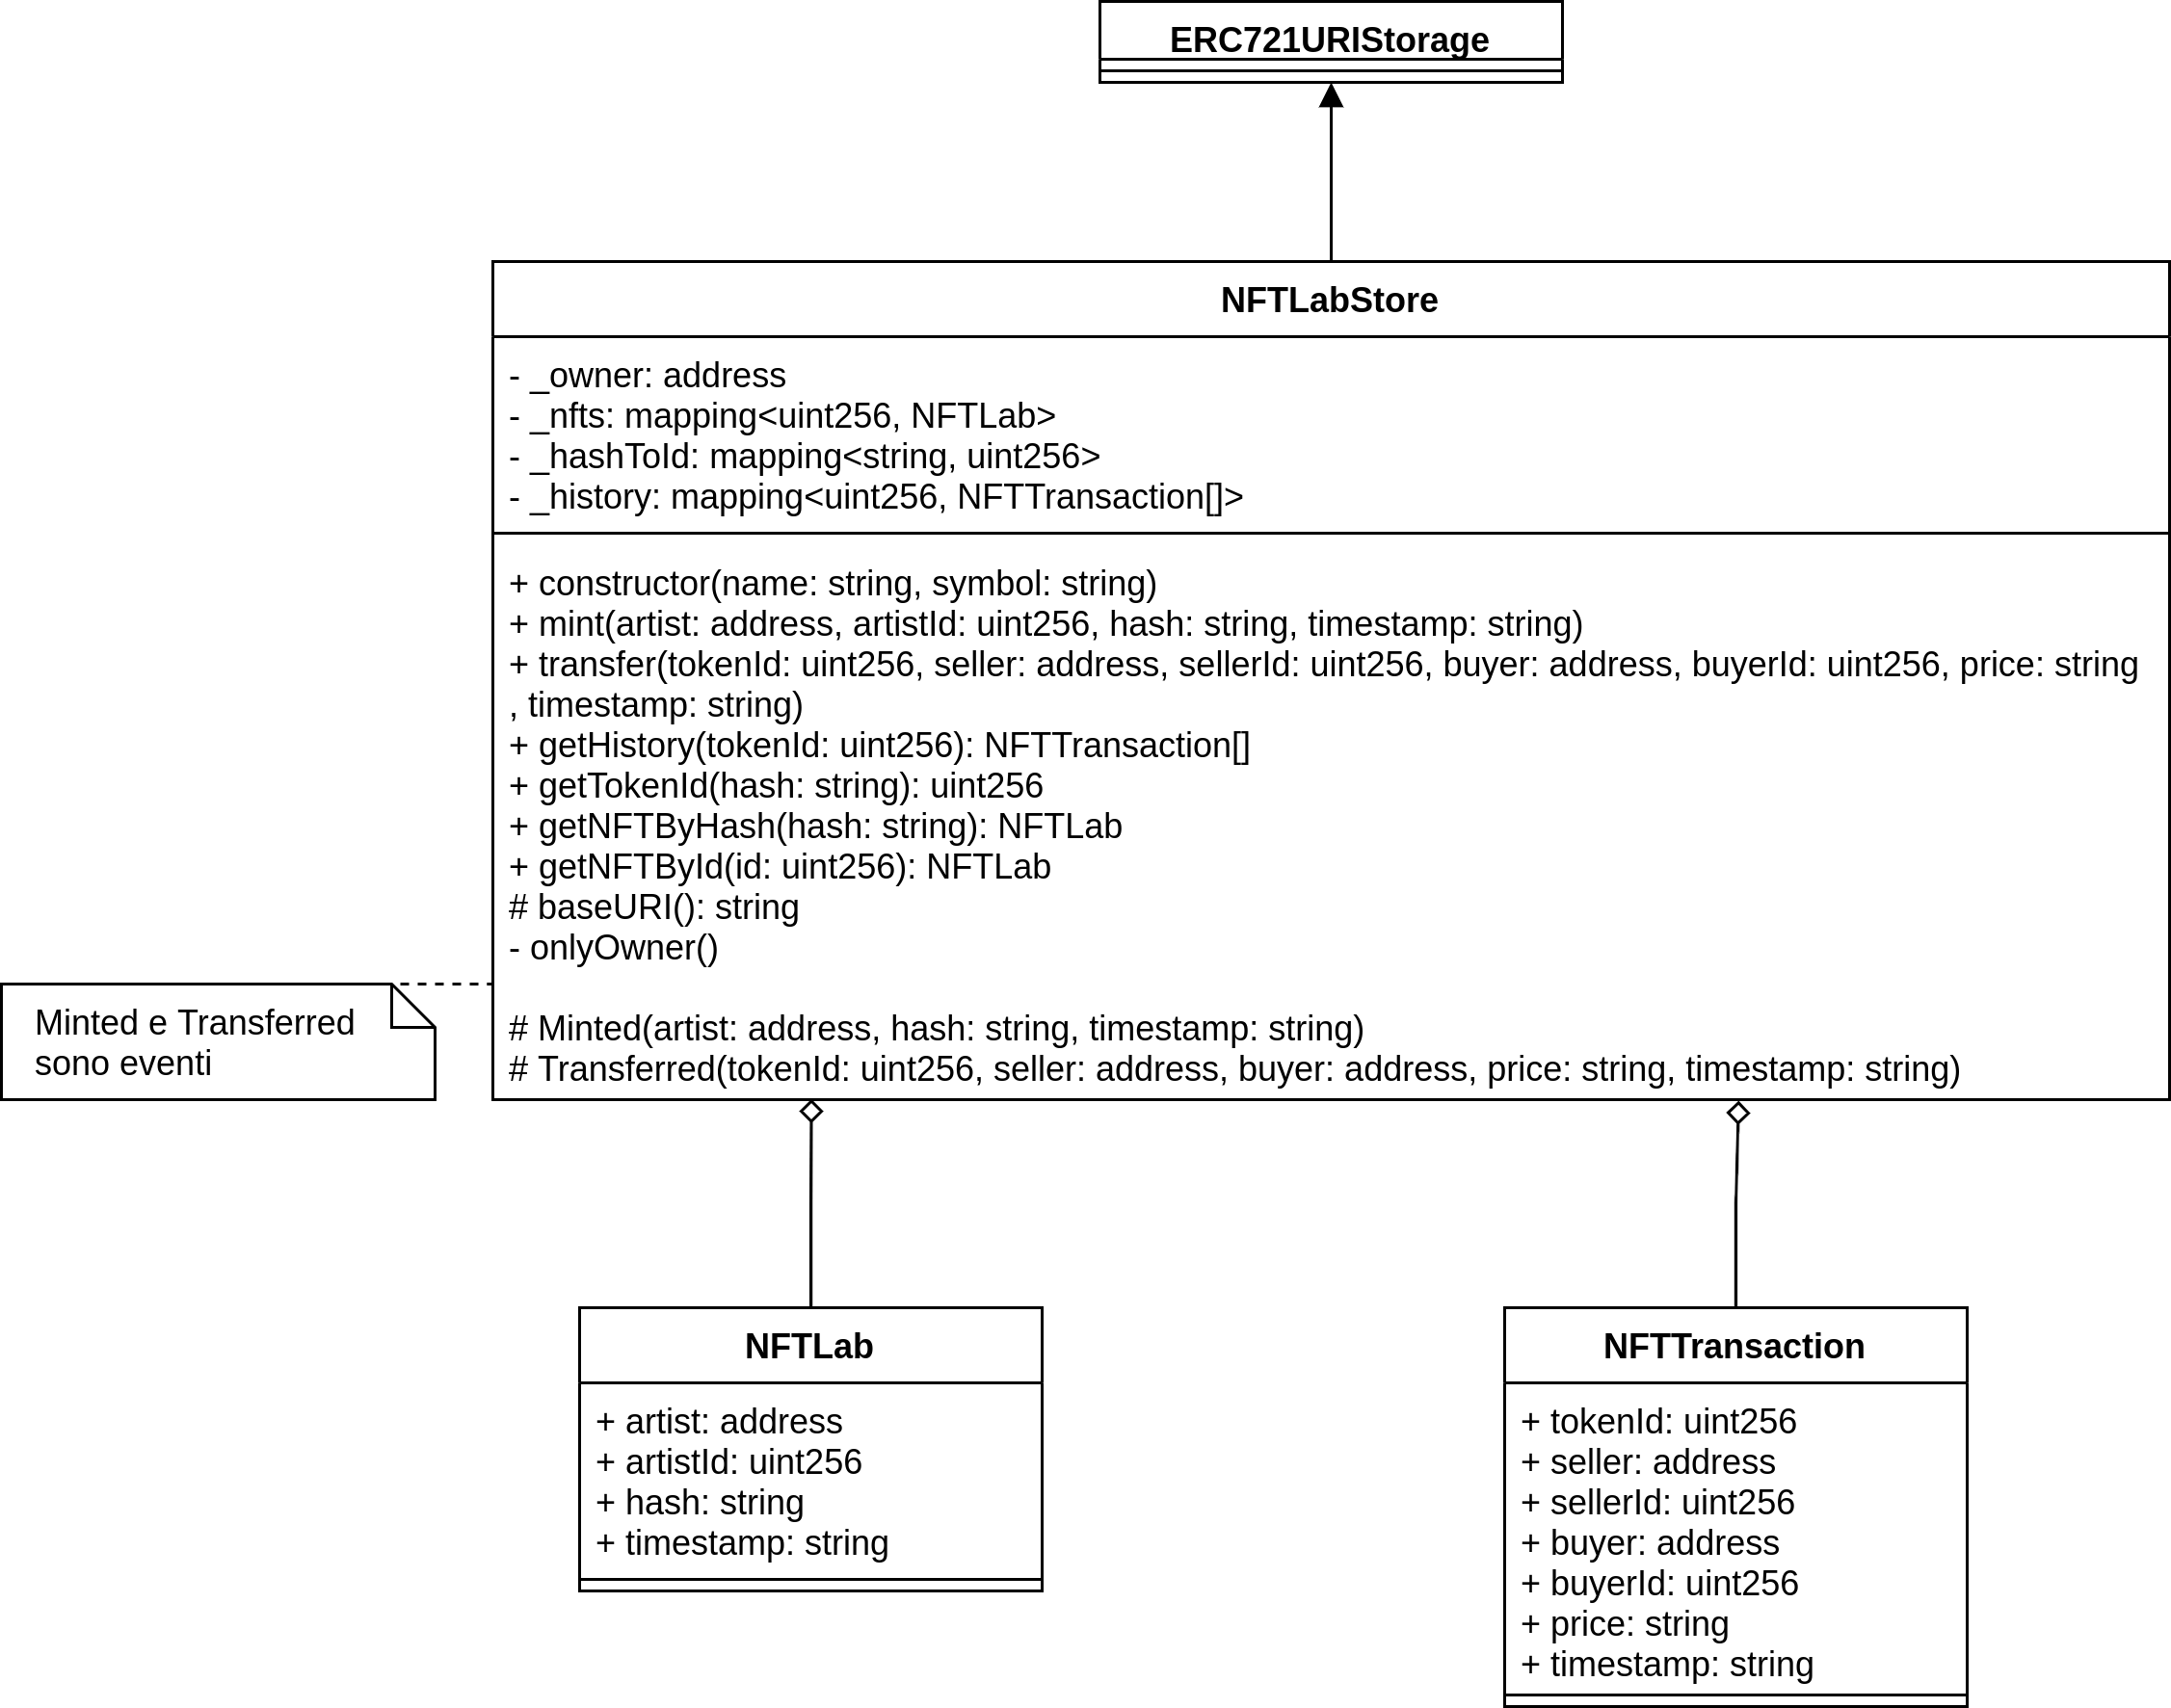
\includegraphics[width=\textwidth]{capitolo3/class-diagram/smart-contract-ethereum-class-diagram.png}
  \caption{Diagramma delle classi dello \textit{smart contract} per Ethereum}
\end{figure}

Il contratto \textit{NFTLabStore} eredita direttamente dal contratto \textit{ERC721URIStorage}, permettendo così anche la memorizzazione del CID di IPFS. Inoltre, sono state utilizzate due strutture dove andare a memorizzare i dati del NFT e delle transazioni. Dato che per l'integrazione da Java è stata utilizzata la libreria Web3J, ho dovuto seguire anche le sue convezioni, in particolare quella dove tutti i metodi che modificano lo stato del contratto non devono ritornare alcun dato.

\subsection{Codifica}
Ultimata la progettazione architetturale dei principali componenti del sistema, è iniziata la fase di codifica nella quale ho semplicemente implementato quanto ottenuto dalla progettazione. Ho sviluppato il contratto scrivendo prima le firme di tutto quello che era richiesto, per poi implementare.

\clearpage
convezione
\begin{figure}[h!]
  \centering
  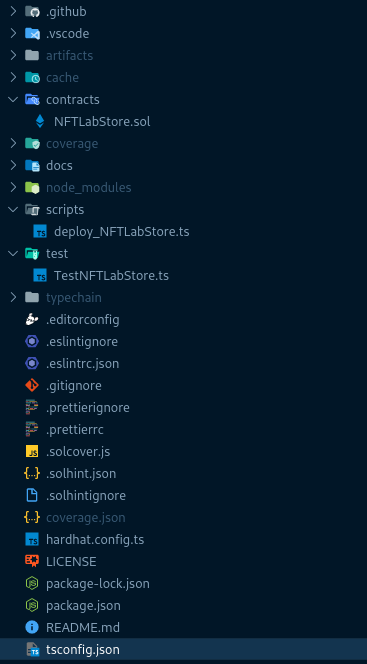
\includegraphics[width=0.3\textwidth]{capitolo3/smart-contract-ethereum/smart-contract-ethereum-structure.png}
  \caption{Struttura del progetto del contratto per Solidity}
\end{figure}

Durante la fase di codifica sono stato molto attento a seguire le \textit{best practices} e le convezioni date dal linguaggio Solidity. In particolare:
\begin{itemize}
  \item tutte le funzioni che non modificano lo stato sono state segnate come \textit{view};
  \item utilizzo di variabili \textit{memory} per tutti gli oggetti che non devono essere memorizzati.
\end{itemize}

Meritevole di attenzione è sicuramente l'implementazione del \textit{design pattern Access Restriction}. Come si può vedere nel costruttore viene assegnata una variabile, la quale specifica che chi ha eseguito il \textit{deploy} del contratto è il proprietario. In seguito viene creato un modificatore che permette di limitare l'esecuzione di determinate funzioni solo al proprietario.

\begin{figure}[h!]
  \centering
  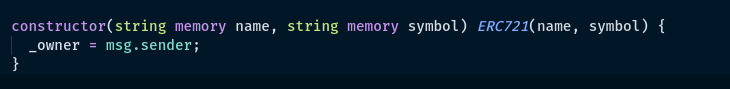
\includegraphics[width=0.8\textwidth]{capitolo3/smart-contract-ethereum/smart-contract-ethereum-constructor.png}
  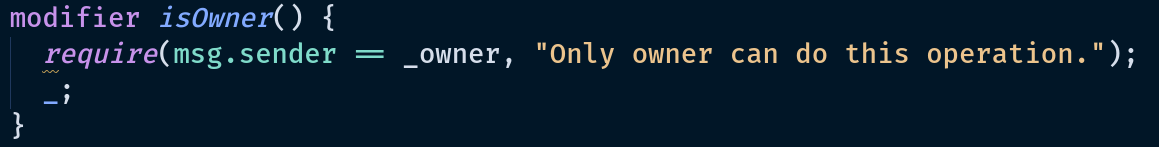
\includegraphics[width=0.8\textwidth]{capitolo3/smart-contract-ethereum/smart-contract-ethereum-modifier.png}
  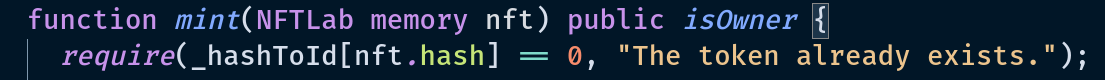
\includegraphics[width=0.8\textwidth]{capitolo3/smart-contract-ethereum/smart-contract-ethereum-modifier-usage.png}
  \caption{Realizzazione del \textit{design pattern Access Restriction} in Solidity}
\end{figure}

\subsection{Verifica}
In parallelo con l'attività di codifica, ho verificato lo sviluppo del contratto sfruttando il \textit{framework} Mocha e la libreria Chai. Questi ultimi si integrano perfettamente con lo strumento HardHat, permettendo, la scrittura di tutti questi test attraverso il linguaggio Typescript. Dato che lo \textit{smart contract} può essere eseguito solamente su \textit{blockchain}, HardHat provvederà ad eseguire il \textit{deploy} di quest'ultimo in una \textit{blockchain} temporanea dove verranno eseguiti tutti i \textit{test}. 

Questo avviene tramite una libreria ed uno strumento aggiuntivo per HardHat, ovvero Ether.js e \textit{Typechain}. Ether.js è una libreria per l'interazione con lo \textit{smart contract} da \textit{software} scritti in Javascript. HardHat, durante la fase di compilazione, genera automaticamente i gli ABI del contratto che \textit{Typechain}, in fase di test, utilizzerà per la generazione di file Typescript che hanno il compito di interagire, grazie a Ether.js, con il contratto caricato. In seguito questi file verranno richiamati per eseguire e verificare le varie parti del contratto.

Per quanto riguarda i tipi di test eseguiti, gli unici che sono stati sviluppati sono quelli di unità, perché non potevano essere sviluppati altri tipi di \textit{test} per la natura semplice delle funzioni.

\clearpage

\begin{figure}[h!]
  \centering
  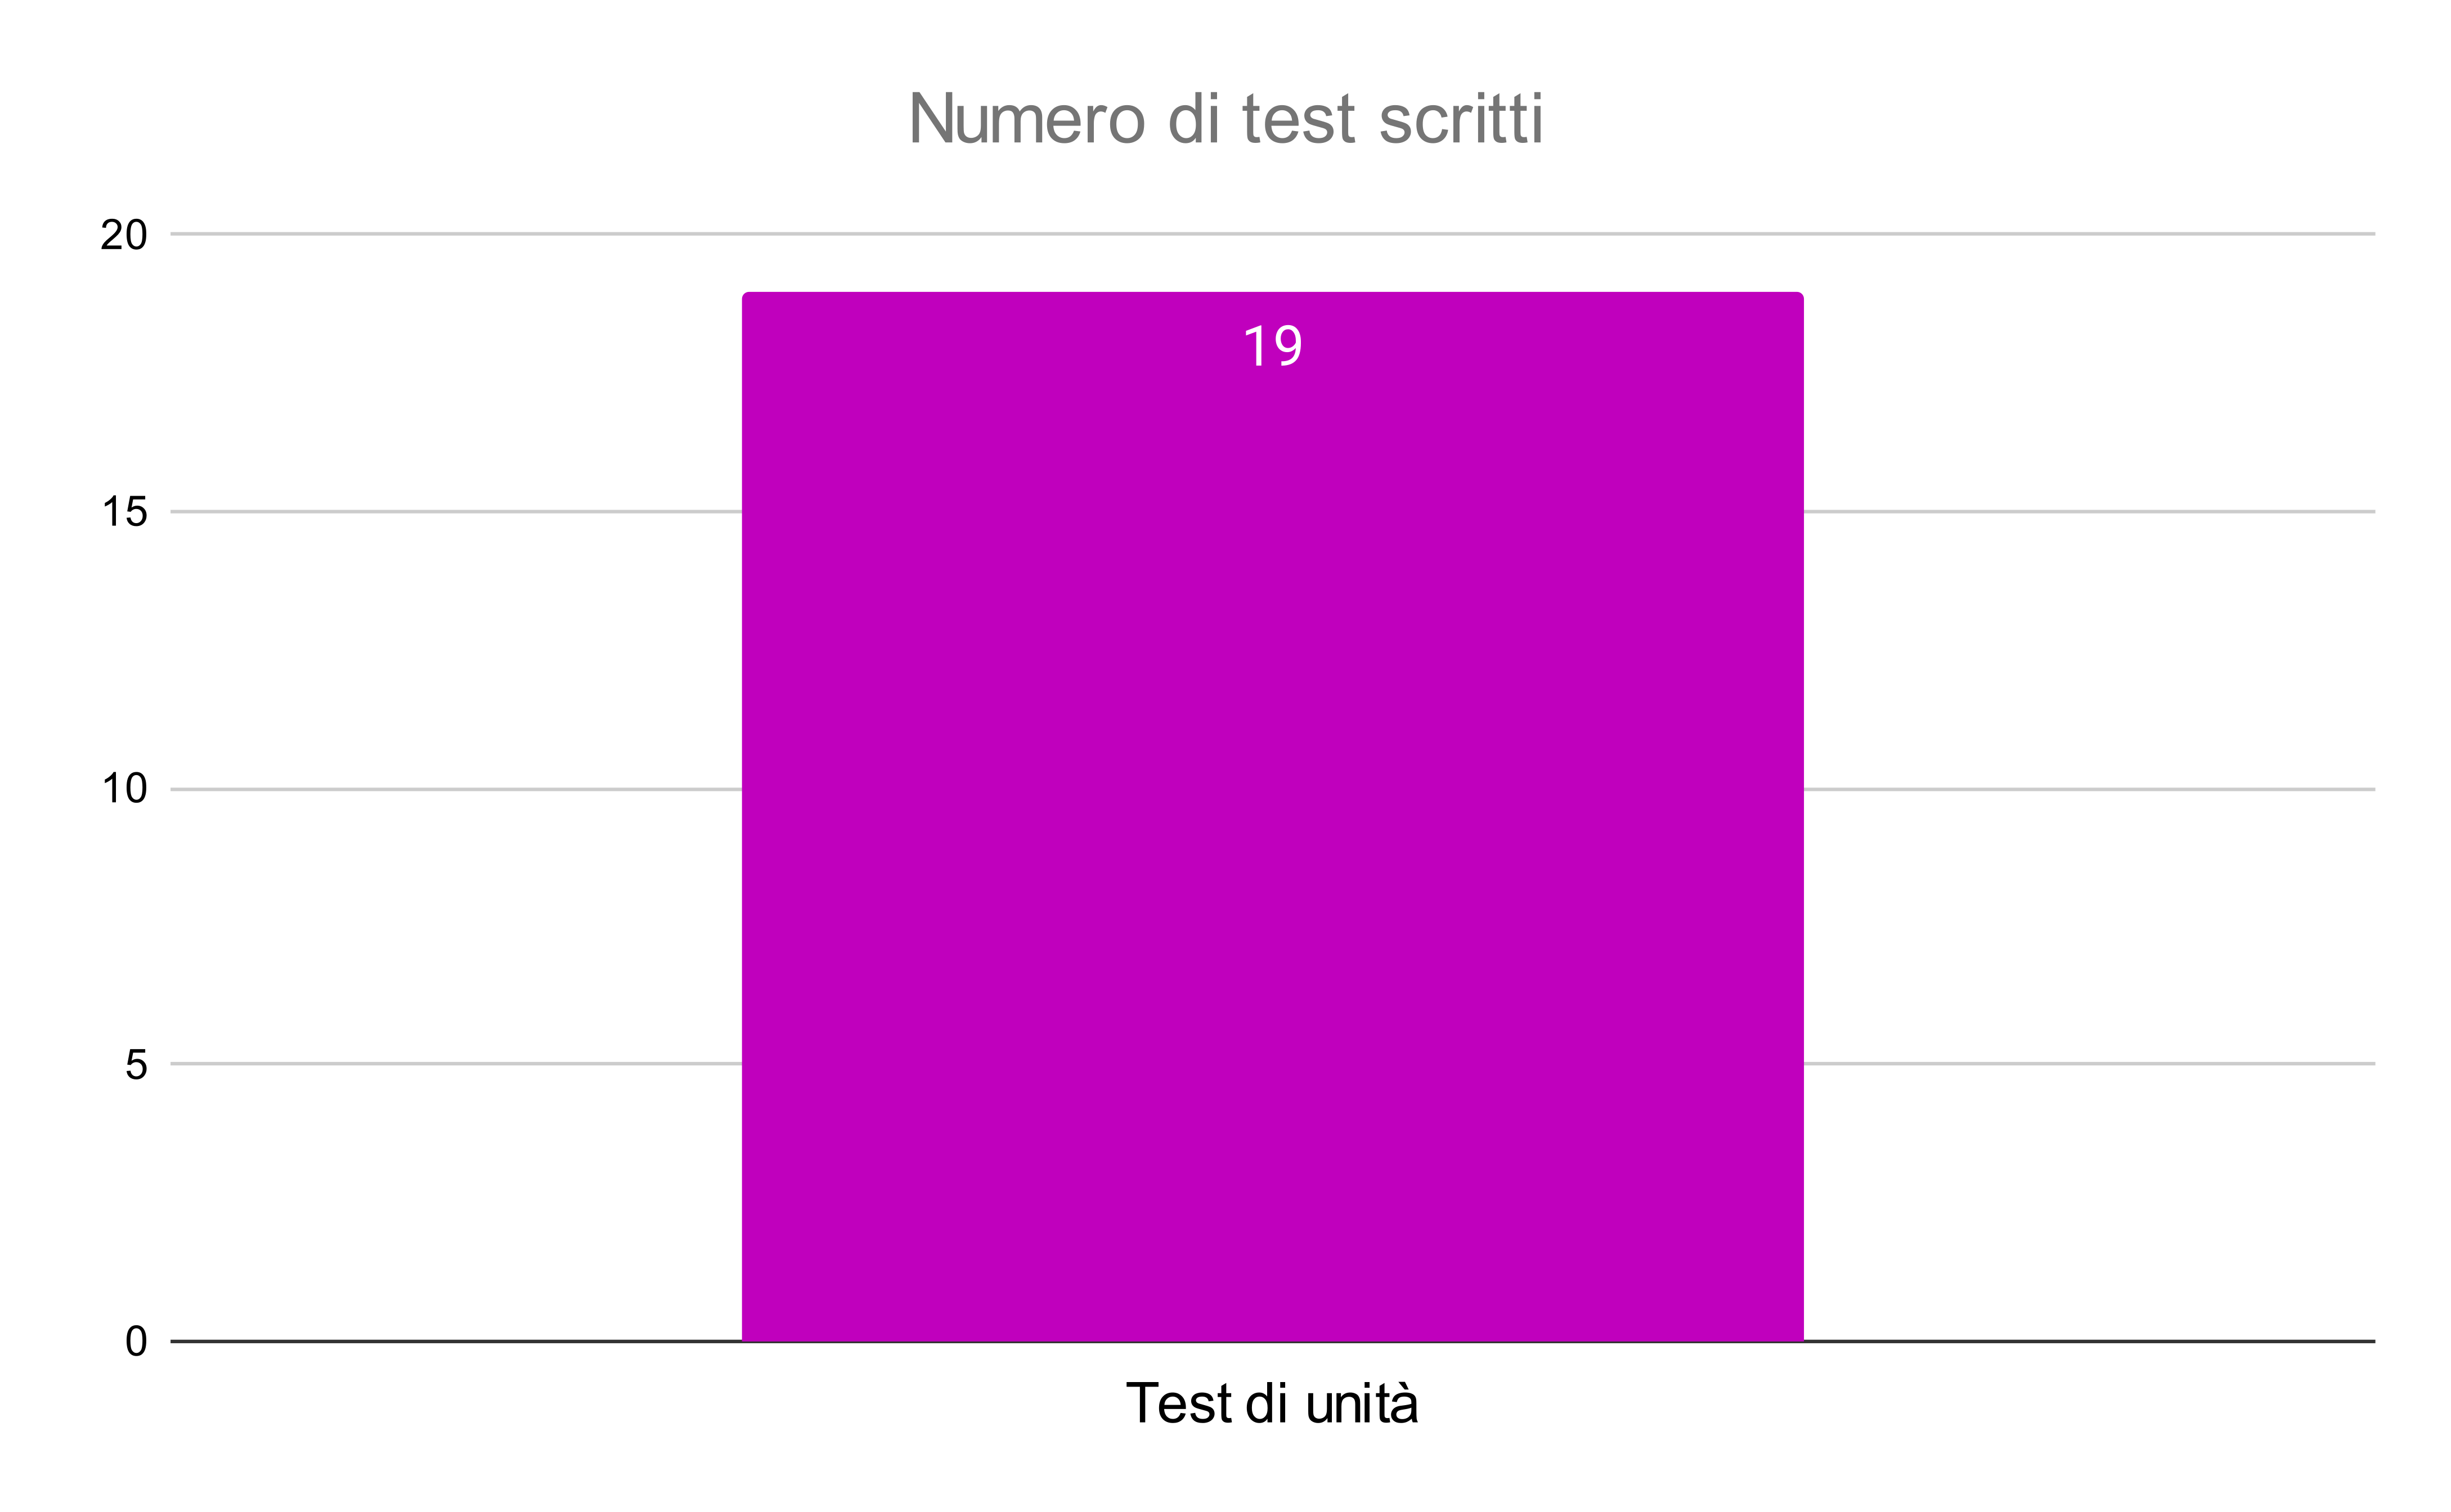
\includegraphics[width=\textwidth]{capitolo3/smart-contract-number-test.png}
  \caption{Numero di test scritti nel contratto in Ethereum}
\end{figure}

In generale, posso affermare che l'attività di verifica si è rilevata molto proficua e mi ha permesso di agevolare lo sviluppo in modo significativo, tanto da produrre un grande quantitativo di \textit{test} e raggiungere un \textit{code coverage} del 100\%.

\clearpage

\begin{figure}[h!]
  \centering
  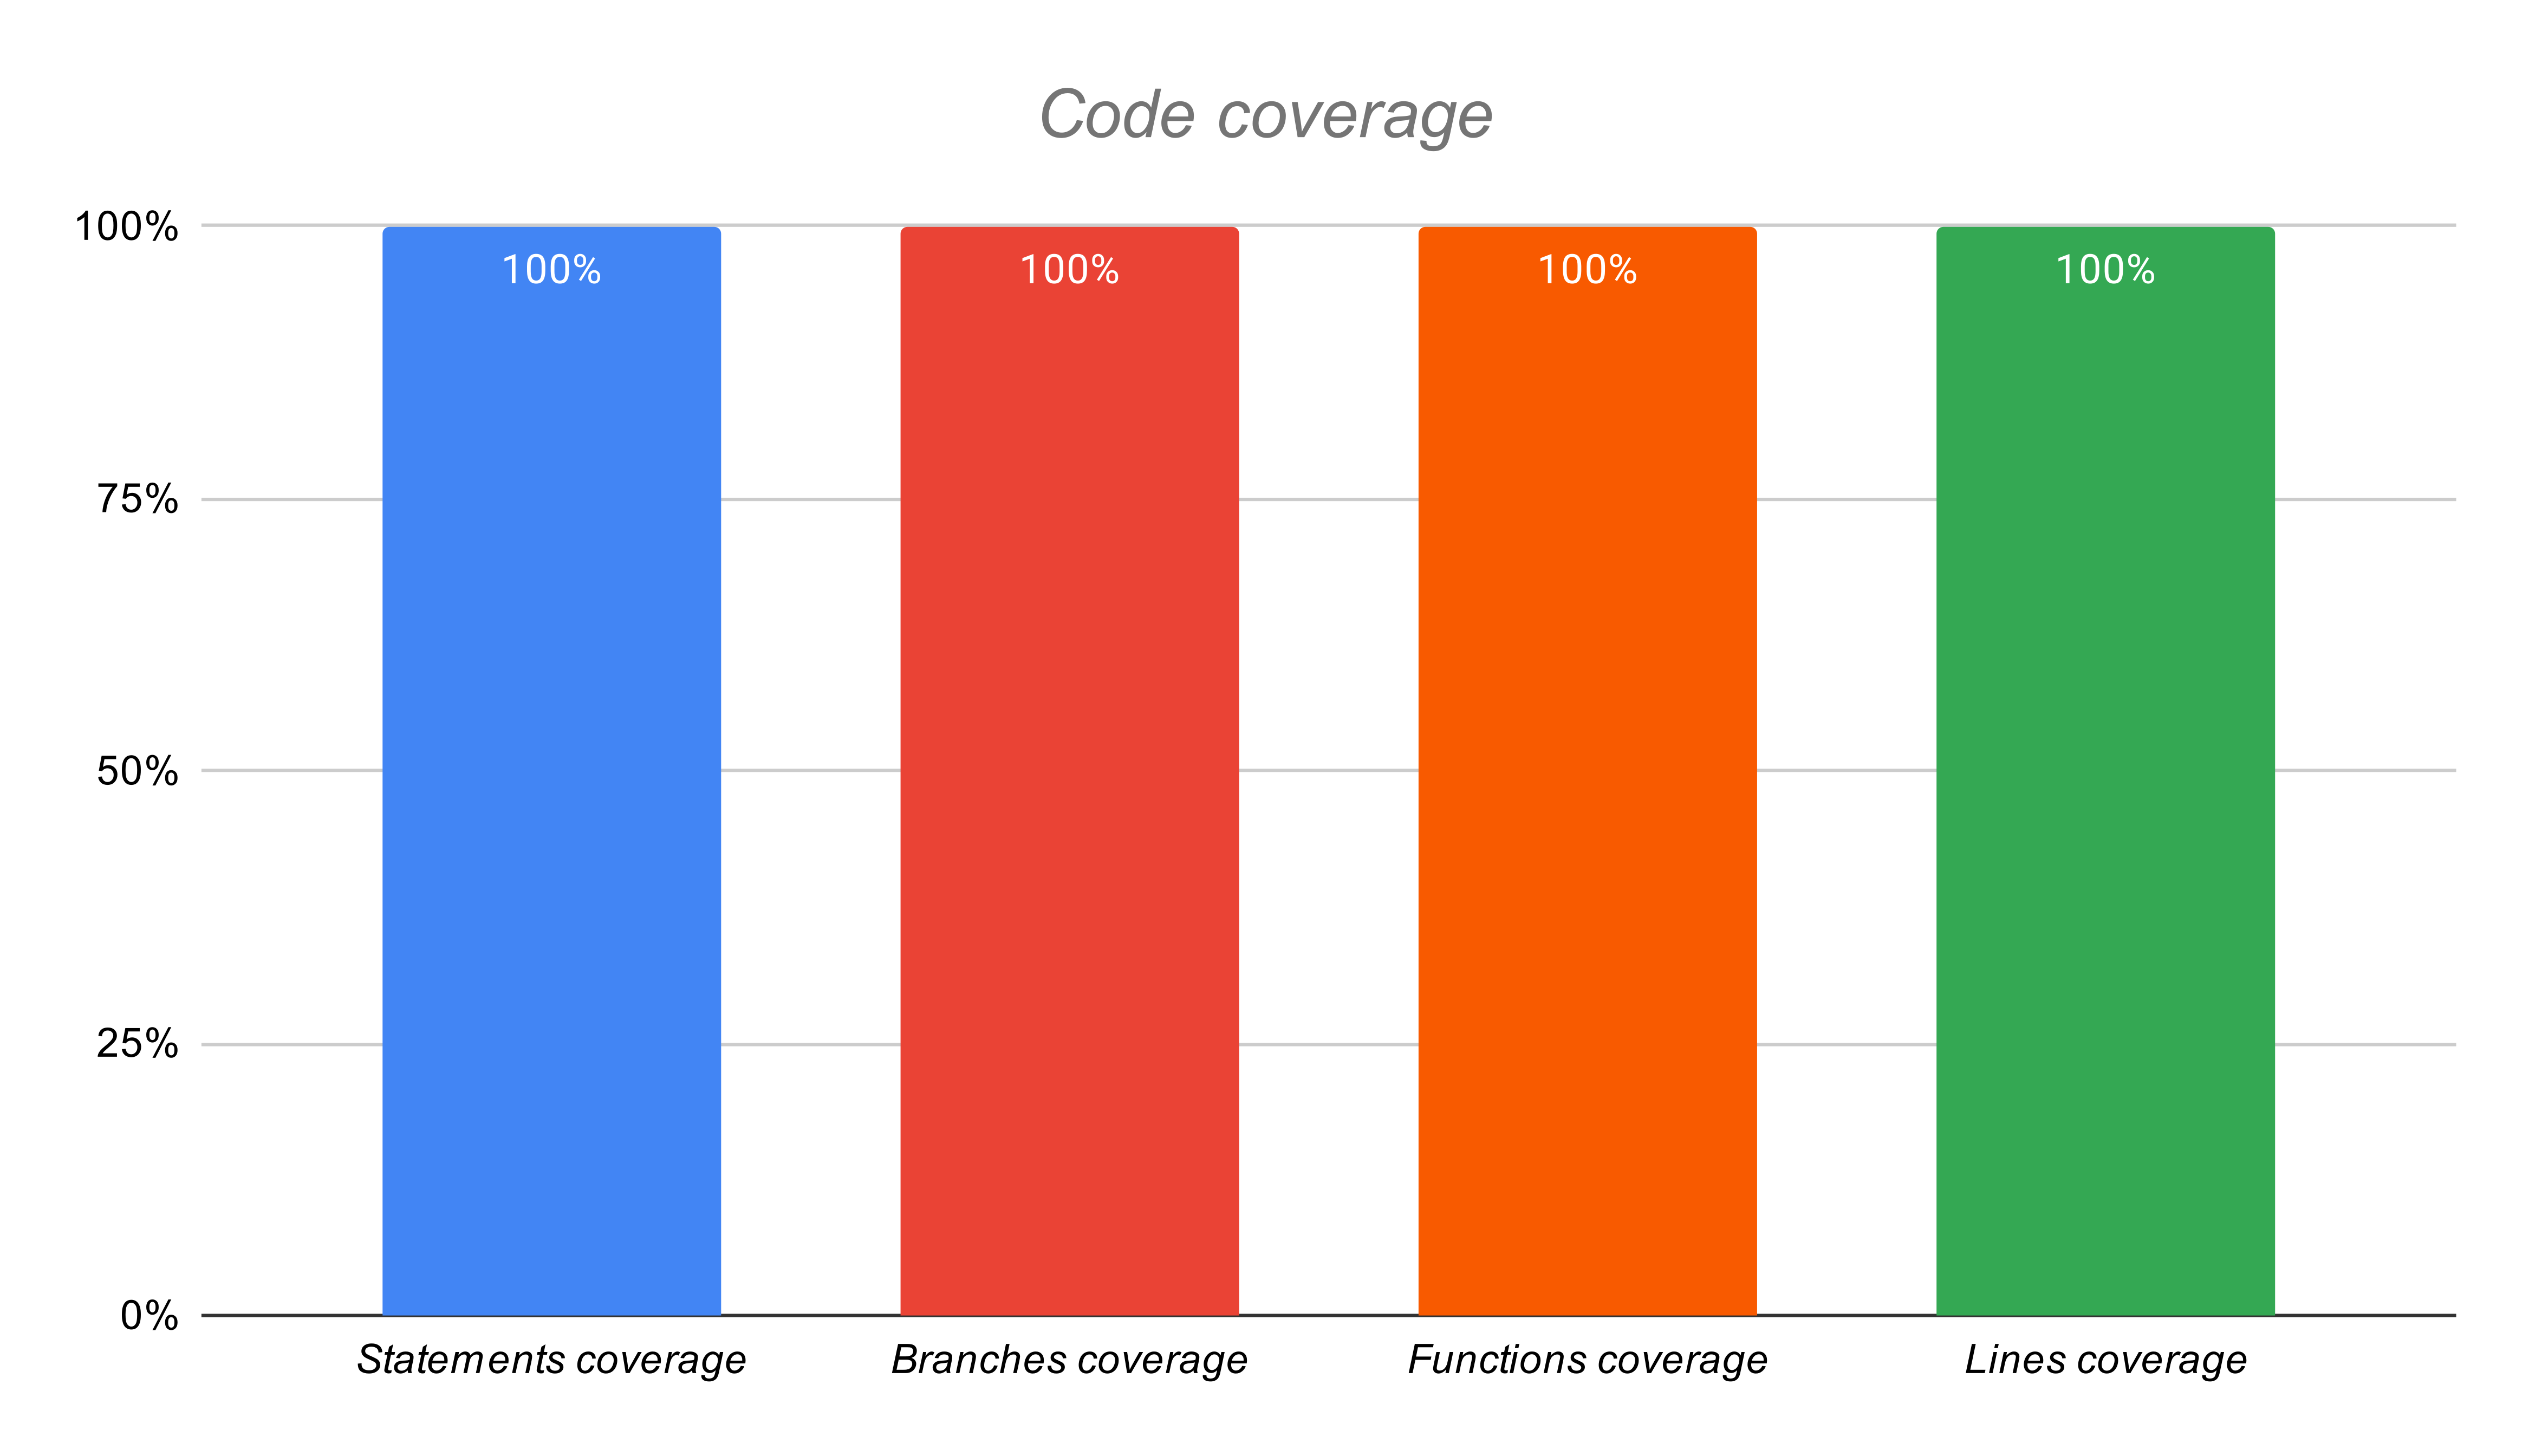
\includegraphics[width=\textwidth]{capitolo3/smart-contract-code-coverage.png}
  \caption{\textit{Code coverage} raggiunto nel contratto in Ethereum}
\end{figure}


%%%%%%%%%%%%%%%%%%%%%%%%%%%%%%%%%%%%%%%%%%%%%%%%%%%%%%%%%%%%%%%%%%%%%%%%%%%%%%%%%

\section{Lo standard ERC721 per Hotmoka}
Spiegazione del perché è risultata necessaria la scrittura dello standard ERC721 per Hotmoka.

\subsection{Progettazione}
Scelte progettuali, best practices impiegate e design pattern che sono stati utilizzati. 

\subsubsection{Architettura}
Presentazione dell'architettura con diagrammi di package, classe e sequenza.

\subsection{Codifica}
Spiegazione di quanto fatto durante il periodo di codifica, approfondendo parti di codice che ritengo importanti.

\subsection{Verifica}
Spiegazione delle librerie attraverso le quali sono stati implementati i test, numero di test scritti e code coverage raggiunto.

%%%%%%%%%%%%%%%%%%%%%%%%%%%%%%%%%%%%%%%%%%%%%%%%%%%%%%%%%%%%%%%%%%%%%%%%%%%%%%%%%

\section{Smart contract per Hotmoka}
Spiegazione dello scopo e dei compiti dello smart contract per Hotmoka.

\subsection{Progettazione}
Scelte progettuali, best practices impiegate e design pattern che sono stati utilizzati. 

\subsubsection{Architettura}
Presentazione dell'architettura con diagrammi di package, classe e sequenza.

\subsection{Codifica}
Spiegazione di quanto fatto durante il periodo di codifica, approfondendo parti di codice che ritengo importanti.

\subsection{Verifica}
Spiegazione delle librerie attraverso le quali sono stati implementati i test, numero di test scritti e code coverage raggiunto.

%%%%%%%%%%%%%%%%%%%%%%%%%%%%%%%%%%%%%%%%%%%%%%%%%%%%%%%%%%%%%%%%%%%%%%%%%%%%%%%%%

\section{Libreria per l'integrazione con gli smart contract}
Spiegazione dello scopo e dei compiti della libreria per l'integrazione con gli smart contract.

\subsection{Progettazione}
Scelte progettuali, best practices impiegate e design pattern che sono stati utilizzati. 

\subsubsection{Architettura}
Presentazione dell'architettura con diagrammi di package, classe e sequenza.

\subsection{Codifica}
Spiegazione di quanto fatto durante il periodo di codifica, approfondendo parti di codice che ritengo importanti.

\subsection{Verifica}
Spiegazione delle librerie attraverso le quali sono stati implementati i test, numero di test scritti e code coverage raggiunto.

%%%%%%%%%%%%%%%%%%%%%%%%%%%%%%%%%%%%%%%%%%%%%%%%%%%%%%%%%%%%%%%%%%%%%%%%%%%%%%%%%

\section{Validazione e collaudo}
Riassunto dei requisiti soddisfatti e risultato del collaudo.

% %%%%%%%%%%%%%%%%%%%%%%%%%%%%%%%%%%%%%%%%%%%%%%%%%%%%%%%%%%%%%%%%%%%%%%%%%%%%%%%%%

% \section{Resoconto dei prodotti sviluppati}
% Quantità di prodotti software che sono stati sviluppati (in termini di linee di codice) e numero di documenti prodotti.

% %%%%%%%%%%%%%%%%%%%%%%%%%%%%%%%%%%%%%%%%%%%%%%%%%%%%%%%%%%%%%%%%%%%%%%%%%%%%%%%%%

% \section{Integrazione del prodotto in NFTLab}
% Come quanto è stato implementato si integra all'interno del prodotto NFTLab.

% %%%%%%%%%%%%%%%%%%%%%%%%%%%%%%%%%%%%%%%%%%%%%%%%%%%%%%%%%%%%%%%%%%%%%%%%%%%%%%%%%

% \section{Le conclusioni}
% Considerazioni conclusive sul confronto tra le due blockchain Hotmoka e Ethereum.
